%                      Code_Saturne version 1.3
%                      ------------------------
%
%     This file is part of the Code_Saturne Kernel, element of the
%     Code_Saturne CFD tool.
%
%     Copyright (C) 1998-2008 EDF S.A., France
%
%     contact: saturne-support@edf.fr
%
%     The Code_Saturne Kernel is free software; you can redistribute it
%     and/or modify it under the terms of the GNU General Public License
%     as published by the Free Software Foundation; either version 2 of
%     the License, or (at your option) any later version.
%
%     The Code_Saturne Kernel is distributed in the hope that it will be
%     useful, but WITHOUT ANY WARRANTY; without even the implied warranty
%     of MERCHANTABILITY or FITNESS FOR A PARTICULAR PURPOSE.  See the
%     GNU General Public License for more details.
%
%     You should have received a copy of the GNU General Public License
%     along with the Code_Saturne Kernel; if not, write to the
%     Free Software Foundation, Inc.,
%     51 Franklin St, Fifth Floor,
%     Boston, MA  02110-1301  USA
%
%-----------------------------------------------------------------------
%
%%%%%%%%%%%%%%%%%%%%%%%%%%%%%%%%%%%%%%%%%%%%%%%%%%%%%%%%%%%%%%%%%%%%%%
%                                                                    %
%                                                                    %
%                                                                    %
% Titre :           Code_Saturne tutorial                            %
%                                                                    %
%                                                                    %
%                                                                    %
%%%%%%%%%%%%%%%%%%%%%%%%%%%%%%%%%%%%%%%%%%%%%%%%%%%%%%%%%%%%%%%%%%%%%%
\documentclass[a4paper,10pt,twoside]{report}

%
%%%%%%%%%%%%%%%%%%%%%%%%%%%%%%%%%%%%%%%%%%%%%%%%%%%%%%%%%%%%%%%%%%%%%%
% PACKAGES OBLIGATOIRES
\usepackage{../../style/csdoc}
%
%%%%%%%%%%%%%%%%%%%%%%%%%%%%%%%%%%%%%%%%%%%%%%%%%%%%%%%%%%%%%%%%%%%%%%

%
%%%%%%%%%%%%%%%%%%%%%%%%%%%%%%%%%%%%%%%%%%%%%%%%%%%%%%%%%%%%%%%%%%%%%%
% PACKAGES ET COMMANDES POUR LE DOCUMENTS PDF ET LES HYPERLIENS
\usepackage[pdftex,
            bookmarksopen=true,
            colorlinks=true,
            linkcolor=blue,
            filecolor=blue,
            urlcolor=blue,
            citecolor=blue]{hyperref}
\hypersetup{%
  pdftitle = {Code_Saturne version 1.3 tutorial},
  pdfauthor = {MFEE},
  pdfpagemode = UseOutlines
}
\pdfinfo{/CreationDate (D:20030429000000-01 00 )}
%
% Pour avoir les Thumbnails a l'ouverture du document sous ACROREAD :
% pdfpagemode = UseThumbs
%
%%%%%%%%%%%%%%%%%%%%%%%%%%%%%%%%%%%%%%%%%%%%%%%%%%%%%%%%%%%%%%%%%%%%%%
% MACROS SUPPLEMENTAIRES
% \newcommand{/...}{...}
%
\renewcommand{\thefigure}{\Roman{part}.\arabic{figure}}
\renewcommand{\thetable}{\Roman{part}.\arabic{table}}
\renewcommand{\theequation}{\Roman{part}.\arabic{equation}}
\renewcommand{\thesection}{\arabic{section}}
%
% repertoire et extension des images
\newcommand{\repgraphics}{../graphics}
\newcommand{\extgraphics}{pdf}
%
%
%%%%%%%%%%%%%%%%%%%%%%%%%%%%%%%%%%%%%%%%%%%%%%%%%%%%%%%%%%%%%%%%%%%%%%

%
%%%%%%%%%%%%%%%%%%%%%%%%%%%%%%%%%%%%%%%%%%%%%%%%%%%%%%%%%%%%%%%%%%%%%%
% INFO POUR PAGES DE GARDES
\titreCS{\CS\ version~\verscs\ tutorial}
\docassociesCS{}
\resumeCS{}
%
%%%%%%%%%%%%%%%%%%%%%%%%%%%%%%%%%%%%%%%%%%%%%%%%%%%%%%%%%%%%%%%%%%%%%%

%
%%%%%%%%%%%%%%%%%%%%%%%%%%%%%%%%%%%%%%%%%%%%%%%%%%%%%%%%%%%%%%%%%%%%%%
% DEBUT DU DOCUMENT
\begin{document}
\pdfgraphics
\def\contentsname{\textbf{\normalsize TABLE OF CONTENTS}\pdfbookmark[1]{Table of
contents}{contents}}
\def\indexname{Index of the main variables and keywords}

\pdfbookmark[1]{Flyleaf}{pdg}
\large
\makepdgCS
\normalsize

\begin{center}\begin{singlespace}
\tableofcontents
\end{singlespace}\end{center}

%
%%%%%%%%%%%%%%%%%%%%%%%%%%%%%%%%%%%%%%%%%%%%%%%%%%%%%%%%%%%%%%%%%%%%%%

%
%%%%%%%%%%%%%%%%%%%%%%%%%%%%%%%%%%%%%%%%%%%%%%%%%%%%%%%%%%%%%%%%%%%%%%
% CORPS DU DOCUMENT
%
\passepage
\stepcounter{chapter}
\part{INTRODUCTION}
%
%                      Code_Saturne version 1.3
%                      ------------------------
%
%     This file is part of the Code_Saturne Kernel, element of the
%     Code_Saturne CFD tool.
%
%     Copyright (C) 1998-2008 EDF S.A., France
%
%     contact: saturne-support@edf.fr
%
%     The Code_Saturne Kernel is free software; you can redistribute it
%     and/or modify it under the terms of the GNU General Public License
%     as published by the Free Software Foundation; either version 2 of
%     the License, or (at your option) any later version.
%
%     The Code_Saturne Kernel is distributed in the hope that it will be
%     useful, but WITHOUT ANY WARRANTY; without even the implied warranty
%     of MERCHANTABILITY or FITNESS FOR A PARTICULAR PURPOSE.  See the
%     GNU General Public License for more details.
%
%     You should have received a copy of the GNU General Public License
%     along with the Code_Saturne Kernel; if not, write to the
%     Free Software Foundation, Inc.,
%     51 Franklin St, Fifth Floor,
%     Boston, MA  02110-1301  USA
%
%-----------------------------------------------------------------------
%
%%%%%%%%%%%%%%%%%%%%%%%%%%%%%%%%%%%%%%%%%%%%%%%%%%%%%%%%%%%%%%%%%%%%%%
% SYNTH�SE
\section{Introduction}

\CS is a system designed to solve the Navier-Stokes
equations in the cases of 2D, 2D axisymmetric or 3D flows. Its main module is
designed for the simulation of flows which may be steady or
unsteady, laminar or turbulent, incompressible or potentially dilatable,
isothermal or not. Scalars and turbulent fluctuations of scalars can be taken into
account. The code includes specific modules, referred to as ``specific physics'',
for the treatment of lagrangian particle tracking, semi-transparent radiative transfer,
gas, pulverized coal and heavy fuel oil combustion,
electricity effects (Joule effect and electric arcs) and compressible flows.
The code also includes an engineering module, Matisse, for the simulation of nuclear waste
surface storage.\\
\CS relies on a finite volume discretization and allows the use of
various mesh types which may be hybrid (containing several kinds of
elements) and may have structural non-conformities (hanging nodes).

The present document is a tutorial for \CS version \verscs.
It presents five simple test cases and guides the future \CS user step by step
into the preparation and the computation of the cases.

The test case directories, containing the necessary meshes and data
are available in the \CS Kernel directory:\\
\texttt{\$CS\_HOME/doc/TUTORIAL/TEST\_CASES}

This tutorial focuses on the procedure and the preparation of the \CS
computations. For more elements on the structure of the code and the definition
of the different variables, it is higly recommended to refer to the user
manual.

\CS is free software; you can redistribute it
and/or modify it under the terms of the GNU General Public License
as published by the Free Software Foundation; either version 2 of
the License, or (at your option) any later version.
\CS is distributed in the hope that it will be
useful, but WITHOUT ANY WARRANTY; without even the implied warranty
of MERCHANTABILITY or FITNESS FOR A PARTICULAR PURPOSE.  See the
GNU General Public License for more details.
%
%%%%%%%%%%%%%%%%%%%%%%%%%%%%%%%%%%%%%%%%%%%%%%%%%%%%%%%%%%%%%%%%%%%%%%

\setcounter{section}{0}
\stepcounter{chapter}
\part{SIMPLE JUNCTION TEST CASE}
%-------------------------------------------------------------------------------

% This file is part of Code_Saturne, a general-purpose CFD tool.
%
% Copyright (C) 1998-2011 EDF S.A.
%
% This program is free software; you can redistribute it and/or modify it under
% the terms of the GNU General Public License as published by the Free Software
% Foundation; either version 2 of the License, or (at your option) any later
% version.
%
% This program is distributed in the hope that it will be useful, but WITHOUT
% ANY WARRANTY; without even the implied warranty of MERCHANTABILITY or FITNESS
% FOR A PARTICULAR PURPOSE.  See the GNU General Public License for more
% details.
%
% You should have received a copy of the GNU General Public License along with
% this program; if not, write to the Free Software Foundation, Inc., 51 Franklin
% Street, Fifth Floor, Boston, MA 02110-1301, USA.

%-------------------------------------------------------------------------------

\section{General description}
%----------------


        \subsection{Objective}
%-----------------------------
The aim of this case is to train the user of \CS on an oversimplified 2D junction
including an inlet, an outlet, walls and symmetries.

        \subsection{Description of the configuration}
%-----------------------------------------------

The configuration is two-dimensional.\\
It consists of a simple junction as shown on figure \ref{figante11}.
The flow enters through a hot inlet into a cold
environment and exits as indicated on the same figure. This geometry can be
considered as a very rough approximation of the cold branch and the downcomer of
the vessel in a nuclear pressurized water reactor. The effect of temperature on
the fluid density is not taken into account in this first example.

\begin{figure}[h!]
\begin{center}
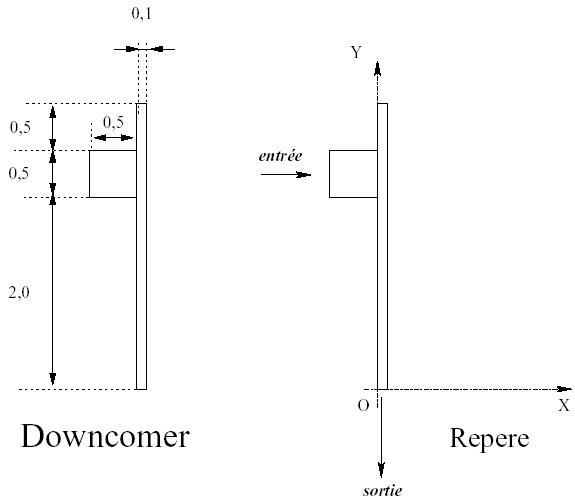
\includegraphics[width=9cm,height=8cm]{fig01}
\caption{Geometry of the downcomer}
\label{figante11}
\end{center}
\end{figure}

        \subsection{Characteristics}
%----------------------------------

Characteristics of the geometry and the flow:
\begin{center}
\begin{tabular}{|l|c|}
\hline
Height of downcomer & $H = 3.00\ m$ \\
\hline
Thickness of downcomer & $E_{d} = 0.10\ m$ \\
\hline
Diameter of the cold branch & $D_{b} = 0.50\ m$ \\
\hline
Inlet velocity of fluid & $V = 1\ m.s^{-1}$ \\
\hline
\end{tabular}\\
\end{center}

Physical characteristics of fluid:\\
The initial water temperature in the domain is equal to 20\degresC.
The inlet temperature of water in the cold branch is 300\degresC.
Water characteristics are considered constant and their values taken at
300\degresC\ and $150\times 10^{5}\ Pa$:
\begin{itemize}
        \item density: $\rho = 725.735\ kg.m^{-3}$
        \item dynamic viscosity: $\mu = 0.895\times10^{-4}\ kg.m^{-1}.s^{-1}$
        \item specific heat: $C_{p} = 5\,483\ J.kg^{-1}.\mbox{\degresC}^{-1}$
        \item Thermal Conductivity $ = 0.02495\ W.m^{-1}.K^{-1}$
\end{itemize}


        \subsection{Mesh characteristics}
%---------------------------------------

Figure \ref{figante12} shows a global view of the downcomer mesh. This
two-dimensional mesh is composed
of 700 cells, which is very small compared to those used in real
studies. This is
a deliberate choice so that tutorial calculations run fast.

\begin{figure}[h!]
\begin{center}
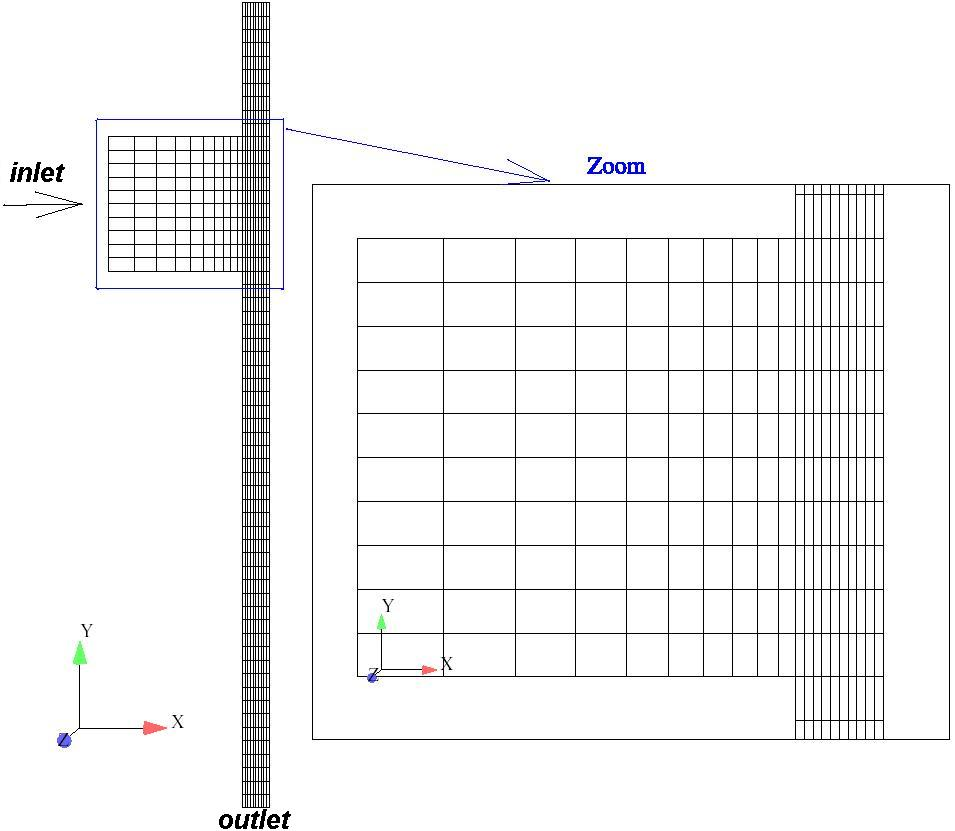
\includegraphics[width=8cm,height=7cm]{fig02}
\caption{Geometry of the downcomer}
\label{figante12}
\end{center}
\end{figure}

Note that here the case is two-dimensional but \CS always operates on three-dimensional
mesh elements (cells). The present mesh is composed of a layer of hexahedrons
created from the 2D mesh shown on figure \ref{figante12} by
extrusion (elevation) in the $Z$ direction. The virtual planes
parallel to $Oxy$ will have ``sliding'' (``symmetry'') conditions to account for
the two-dimensional character of the configuration.\\

{\bfseries Type}: structured mesh

{\bfseries Coordinates system}: cartesian, origin on the edge of the main
pipe at the outlet level, on the nozzle side (figure \ref{figante11})

{\bfseries Mesh generator used}: SIMAIL

{\bfseries Color definition}: see figure \ref{figante13}. To specifiy boundary
conditions on the boundary faces of the mesh, the latter have to be
identified. It is commonly done by assigning an integer to each of them,
characteristic of the boundary region they belong to. This integer is refered to
as "color" or "reference".

\begin{figure}[ht]
\begin{center}
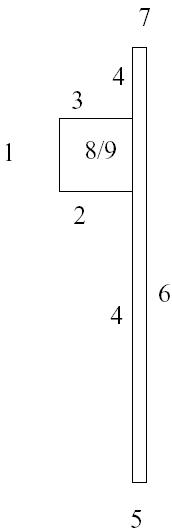
\includegraphics[width=2.5cm,height=6cm]{fig03}
\caption{Colors of the boundary faces}
\label{figante13}
\end{center}
\end{figure}


%-----------------------------------
\section{CASE 1: Basic calculation}
%-----------------------------------

        \subsection{Calculation options}
%-----------------------------------------

Most of the options used in this calculation are default options of \CS.
\begin{itemize}
\renewcommand{\labelitemi}{$\rightarrow$}
        \item Flow type: steady flow
        \item Turbulence model: $k-\epsilon$
        \item Scalar(s): 1 - temperature
        \item Physical properties: uniform and constant
\end{itemize}


        \subsection{Initial and boundary conditions}
%---------------------------------------------------

\begin{itemize}
\renewcommand{\labelitemi}{$\rightarrow$}
        \item Initialization: none (default values)
\end{itemize}


The boundary conditions are defined as follows:
\begin{itemize}
        \item {\bfseries Flow inlet}: Dirichlet condition, an inlet velocity of
$1\ m.s^{-1}$ and an inlet temperature of 300\degresC\ are imposed
        \item {\bfseries Outlet}: default values
        \item {\bfseries Walls}: default values
\end{itemize}

Figure \ref{figante13} shows the colors used for boundary conditions and
table \ref{tabante11} defines the correspondance between the colors and
the type of boundary condition to use.

Do not forget to enter the value of the hydraulic diameter, adapted to the
current inlet (used for turbulence entry conditions).\\

\begin{table}[htp]
\begin{center}
\begin{tabular}{|c|c|}
\hline
Colors & Conditions \\
\hline
1 & Inlet \\
\hline
5 & Outlet \\
\hline
2 3 4 6 7 & Wall \\
\hline
8 9 & Symmetry\\
\hline
\end{tabular}
\caption{\label{tabante11}Boundary conditions and associated references}
\end{center}
\end{table}

        \subsection{Parameters and User routines}
%------------------------------------------------

All parameters necessary to this study can be defined through the Graphical
Interface without using any user Fortran files.

\begin{center}
\begin{tabular}{|l|c|}
\hline
\multicolumn{2}{|c|}{Calculation control parameters} \\
\hline
Number of iterations & $30$ \\
\hline
Relaxation coefficient & $0.9$ \\
\hline
Output period for post-processing files& $1$ \\
\hline
\end{tabular}
\end{center}



        \subsection{Results}
%---------------------------

Figure \ref{fige1_e1} presents the results obtained at different iterations in the
calculation. They were plotted from the post-processing files, with EnSight.

\textbf{Note:} since the ``steady flow'' option has been chosen, the evolution
of the flow iteration after iteration has no physical meaning. It is merely an
indication of the rapidity of convergence towards the (physical) steady state.

\begin{figure}[h]
\parbox{0.5\textwidth}{%
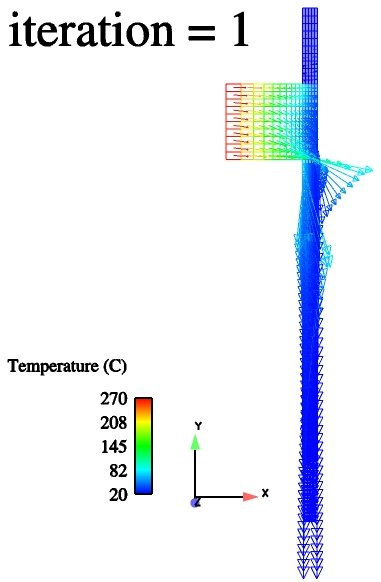
\includegraphics[width=4cm]{cas1_t_1}}
\parbox{0.5\textwidth}{%
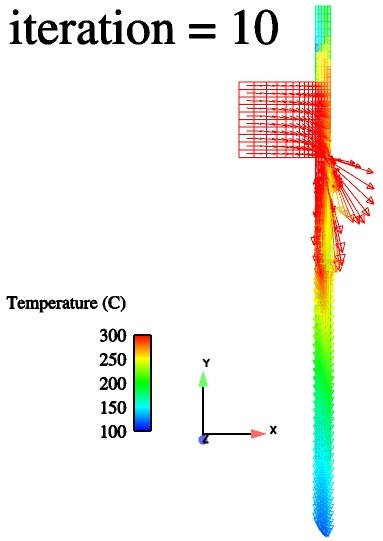
\includegraphics[width=4cm]{cas1_t_10}}
\vspace*{0.5cm}
\parbox{0.5\textwidth}{%
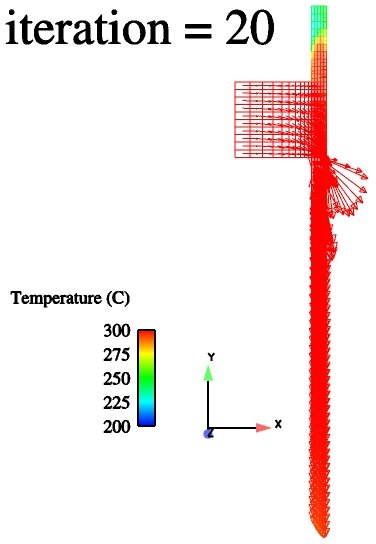
\includegraphics[width=4cm]{cas1_t_20}}
\parbox{0.5\textwidth}{%
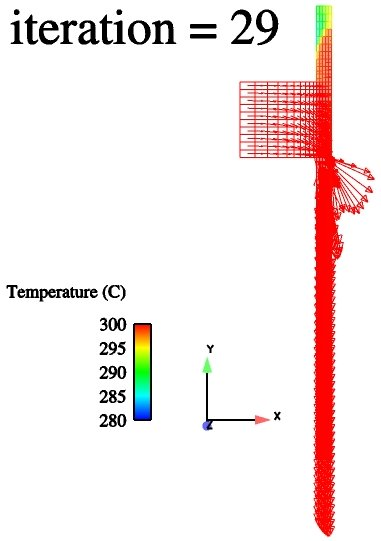
\includegraphics[width=4cm]{cas1_t_29}}
\caption{\label{fige1_e1}Water velocity field colored by temperature at different time steps}
\end{figure}



\setcounter{section}{0}
\stepcounter{chapter}
\part{FULL DOMAIN}
%                      Code_Saturne version 1.3
%                      ------------------------
%
%     This file is part of the Code_Saturne Kernel, element of the
%     Code_Saturne CFD tool.
% 
%     Copyright (C) 1998-2007 EDF S.A., France
%
%     contact: saturne-support@edf.fr
% 
%     The Code_Saturne Kernel is free software; you can redistribute it
%     and/or modify it under the terms of the GNU General Public License
%     as published by the Free Software Foundation; either version 2 of
%     the License, or (at your option) any later version.
% 
%     The Code_Saturne Kernel is distributed in the hope that it will be
%     useful, but WITHOUT ANY WARRANTY; without even the implied warranty
%     of MERCHANTABILITY or FITNESS FOR A PARTICULAR PURPOSE.  See the
%     GNU General Public License for more details.
% 
%     You should have received a copy of the GNU General Public License
%     along with the Code_Saturne Kernel; if not, write to the
%     Free Software Foundation, Inc.,
%     51 Franklin St, Fifth Floor,
%     Boston, MA  02110-1301  USA
%
%-----------------------------------------------------------------------
\section{General description}
%----------------

	\subsection{Objective}
%-----------------------------

This aim of this case is to tackle the merging of initially separate meshes into
a single fluid domain. The questions of mesh pasting and hanging nodes will be
addressed. The test case will then be used to present more complex calculations,
with time dependent variables and Fortran user routines.


	\subsection{Description of the configuration}
%-----------------------------------------------

The fluid domain is composed of three separate meshes, very roughly representing
elements of a nuclear pressurized water reactor vessel: 
\begin{itemize}
	\item the downcomer
	\item the vessel's bottom
	\item the lower core plate and core 
\end{itemize}

Figure \ref{figante21} represents the complete domain. The flow circulates from
the top left horizontal junction to the right vertical outlet. 

\begin{figure}[h!]
\begin{center}
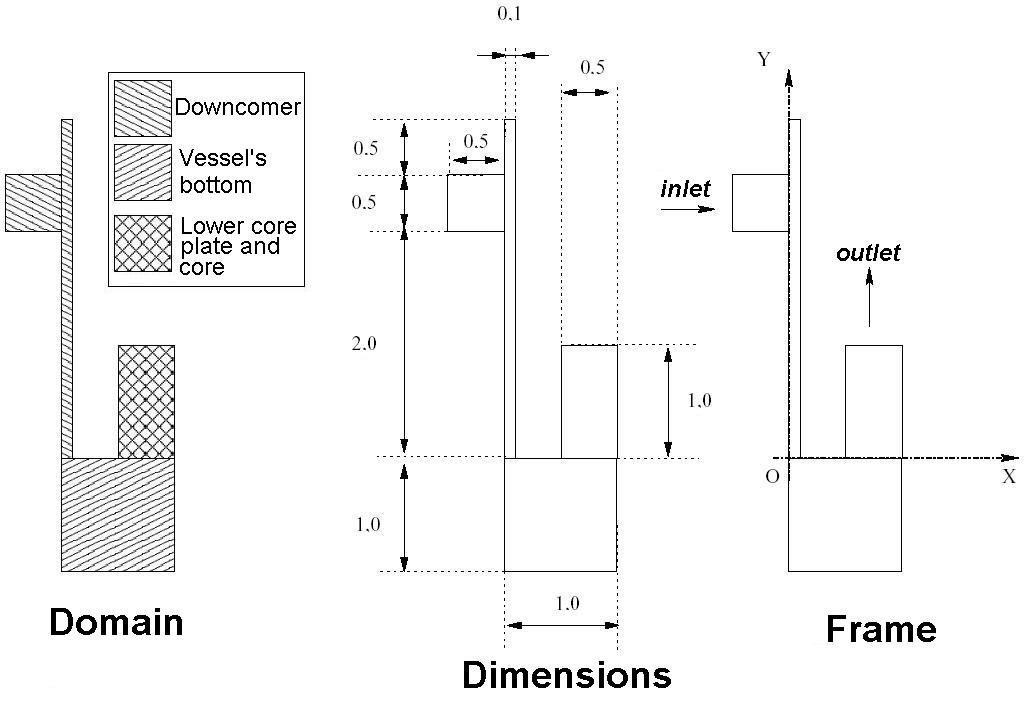
\includegraphics[width=9cm,height=6cm]{\repgraphics/fig04.jpg} 
\caption{Geometry of the complete domain}
\label{figante21}
\end{center}
\end{figure}


	\subsection{Characteristics}
%----------------------------------

The characteristics of the geometry and the flow are:
\begin{center}
\begin{tabular}{|l|c|}
\hline
Height of downcomer & $H = 3.00\ m$ \\
\hline 
Thickness of downcomer & $E_{d} = 0.10\ m$ \\ 
\hline 
Diameter of the inlet cold branch & $D_{b} = 0.50\ m$ \\ 
\hline 
Height of vessel's bottom & $H_{fc} = 1.00\ m$ \\ 
\hline 
Width of vessel's bottom & $l_{fc} = 1.00\ m$ \\ 
\hline 
Height of core above the lower core plate & $H_{pic} = 1.00\ m$ \\ 
\hline 
Width of core above the lower core plate & $l_{pic} = 0.50\ m$ \\ 
\hline 
Inlet velocity of fluid & $V = 1\ m.s^{-1}$ \\ 
\hline 
\end{tabular}\\
\end{center}

Physical characteristics of fluid:\\
The initial water temperature in the domain is equal to 20\degresC.
The inlet temperature of water in the cold branch is 300\degresC.
Water characteristics are considered constant\footnote{which makes temperature a
passive scalar ... but it is only for simplification purposes} and their values taken at
300\degresC\ and $150\times 10^{5}\ Pa$, except density which is considered
variable in cases 3 and 4: 
\begin{itemize}
	\item density: $\rho = 725.735\ kg.m^{-3}$ 
	\item dynamic viscosity: $\mu = 0.895\times10^{-4}\ kg.m^{-1}.s^{-1}$
	\item heat capacity: $C_{p} = 5\,483\ J.kg^{-1}.\mbox{\degresC}^{-1}$ 
\end{itemize}



	\subsection{Mesh characteristics}
%---------------------------------------

Figure \ref{figante22} shows a global view of the mesh and some details of
the pasting zones, to show that \CS\ can deal with hanging nodes.
This mesh is composed of 1\,650 cells, which is very small compared to those used in real
studies. This is a deliberate choice so that tutorial calculations run fast.
	
\begin{figure}[h!]
\begin{center}
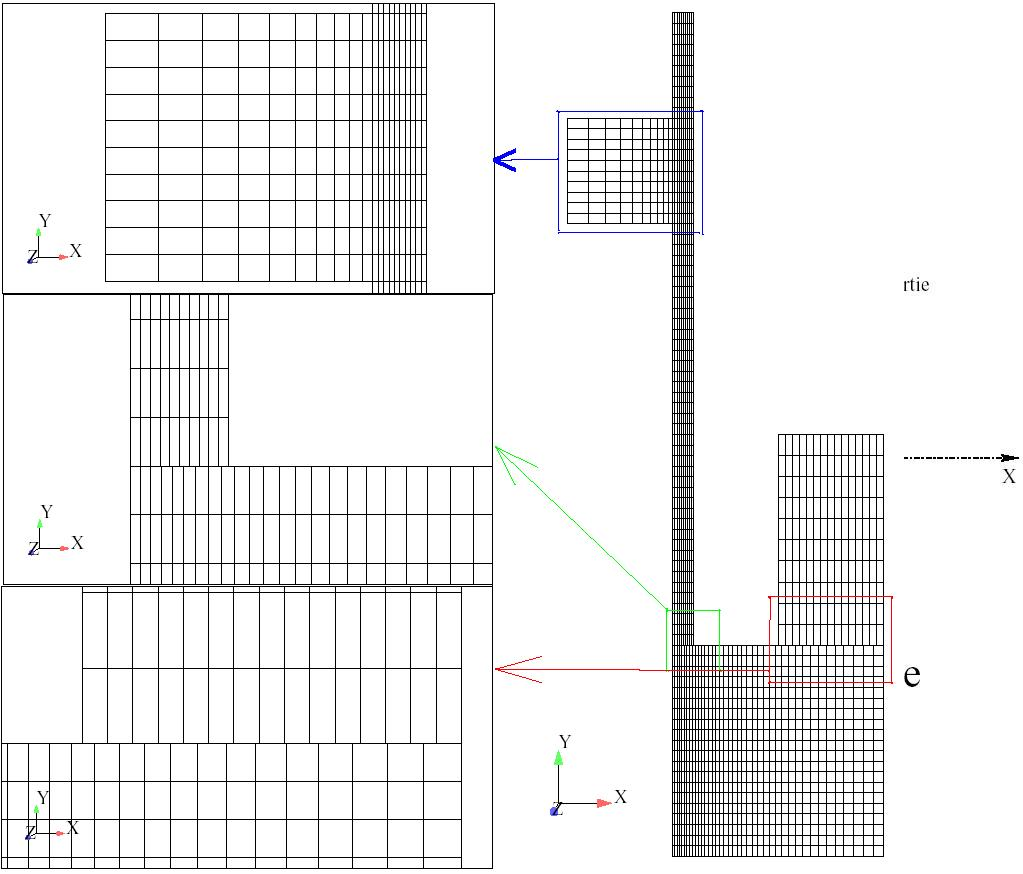
\includegraphics[width=8.65cm,height=7.4cm]{\repgraphics/fig05.jpg} 
\caption{View of the full domain mesh with zoom on the pasting regions}
\label{figante22}
\end{center}
\end{figure}

{\bfseries Type}: block structured mesh

{\bfseries Coordinates system}: cartesian, origin on the edge of the main
pipe at the outlet level, on the nozzle side (figure \ref{figante22})

{\bfseries Mesh generator used}: SIMAIL and mesh pasting with the Preprocessor
of \CS\ (in order to deal with hanging nodes)

{\bfseries Color definition}: see figure \ref{figante23} 

\begin{figure}[h!]
\begin{center}
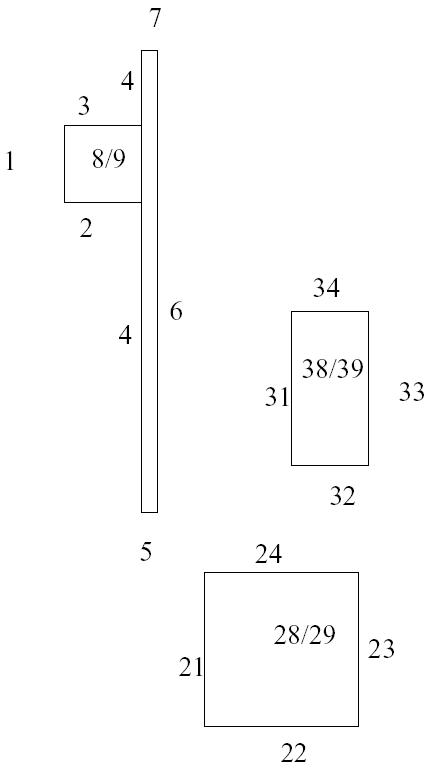
\includegraphics[width=3.6cm,height=6.4cm]{\repgraphics/fig06.jpg} 
\caption{Colors of the boundary faces}
\label{figante23}
\end{center}
\end{figure}


	\subsection{Summary of the different calculations}
%---------------------------------------------------------

Three cases will be studied with this geometry. The following table gives a
summary of their different characteristics.
\begin{center}
\begin{tabular}{|c|c|}
\hline
CASE & characteristics \\
\hline
CASE 2 & unsteady flow, additionnal passive scalar, output management \\
\hline
CASE 3 & same as case 2 with time dependent boundary conditions, \\ 
 &       fluid density depending on the temperature and calculation restart\\
\hline
CASE 4 & same as case 3 with head loss, parallelism and spatial average \\
\hline
\end{tabular}
\end{center}


%--------------------------------------------------------------------------------------
\section{CASE 2: Passive scalar with various boundary conditions and output management}
%--------------------------------------------------------------------------------------

	\subsection{Calculation options}
%-----------------------------------------

Some options are similar to case 1:
\begin{itemize}
\renewcommand{\labelitemi}{$\rightarrow$}
	\item Turbulence model: $k-\epsilon$
	\item Scalar(s): 1 - temperature
	\item Physical properties: uniform and constant
\end{itemize}

The new options are: 
\begin{itemize}
\renewcommand{\labelitemi}{$\rightarrow$}
	\item Flow type: unsteady flow
	\item Time step: uniform and constant
	\item Scalar(s): 2 - passive scalar\footnote{could correspond to a tracer
concentration for instance}
	\item Management of monitoring points
\end{itemize}


	\subsection{Initial and boundary conditions}
%---------------------------------------------------

\begin{itemize}
\renewcommand{\labelitemi}{$\rightarrow$}
	\item Initialization: 20\degresC\ for temperature (default value) \\
	\hspace*{2.1cm}        10 for the passive scalar
\end{itemize}


The boundary conditions are defined in the user interface and depend on the
boundary zone.

\begin{itemize}
	\item {\bfseries Flow inlet}: Dirichlet condition, an inlet velocity of
$1\ m.s^{-1}$, an inlet temperature of 300\degresC\ and an inlet value of 200
for the passive scalar are imposed
	\item {\bfseries Outlet}: default value
	\item {\bfseries Walls}: velocity, pressure and thermal scalar: default value \\
	            \hspace*{1.25cm} passive scalar: different conditions
depending on the color and geometric parameters
\end{itemize}

In order to test the ability to specify boundary condition regions in the
Graphical Interface, various conditions will be imposed for the passive scalar,
as specified in the following table:

\begin{center}
\begin{tabular}{|c|c|c|}
\hline
Wall & Nature & Value \\
\hline 
wall\_1 & Dirichlet  & 0 \\ 
\hline 
wall\_2 & Dirichlet  & 5 \\ 
\hline 
wall\_3 & Dirichlet  & 0 \\ 
\hline 
wall\_4 & Dirichlet  & 25 \\ 
\hline 
wall\_5 & Dirichlet  & 320 \\ 
\hline 
wall\_6 & Dirichlet  & 40 \\ 
\hline
\end{tabular} 
\end{center}

The ``wall\_1'' to ``wall\_6'' regions are defined as follows, through color
references and geometric localization:
\begin{center}
\begin{tabular}{c|c}
Label & Color and geometric parameters \\
\hline
wall\_1 & 24 and $0.1\leqslant X$ and $X\leqslant 0.5$ \\
wall\_2 & 2 or 3 \\
wall\_3 & 4 or 7 or 21 or 22 or 23 \\
wall\_4 & 6 and $Y\leqslant1$ \\
wall\_5 & 6 and $Y>1$ \\
wall\_6 & 31 or 33 \\
\end{tabular}
\end{center}

Figure \ref{figante23} shows the colors used for boundary conditions and 
table \ref{tabante21} defines the correspondance between the colors and  
the type of boundary condition to use.

\begin{table}[htp]
\begin{center}
\begin{tabular}{|c|c|} 
\hline
Colors & Conditions \\
\hline
1 & Inlet \\
\hline
34 & Outlet \\
\hline
2 3 4 6 7 21 22 23 24 31 33 & Wall \\
\hline
8 9 28 29 38 39 & Symmetry \\
\hline
\end{tabular}
\caption{Boundary faces colors and associated references}
\label{tabante21}
\end{center}
\end{table}


	\subsection{Parameters and User routines}
%------------------------------------------------

All parameters necessary to this study can be defined through the Graphical
Interface without using any user Fortran files.

\begin{center}
\begin{tabular}{|l|c|}
\hline
\multicolumn{2}{|c|}{Calculation control parameters} \\
\hline
Number of iterations & $300$ \\
\hline
Reference time step & $0.05$ \\
\hline
Output period for post-processing files& $2$ \\
\hline
\end{tabular}\\
\end{center}

In order to paste the separate meshes into a single domain, colors 5, 24 and 32
will have to be pasted through the Graphical Interface.



	\subsection{Output management}
%-------------------------------------

In this case, different aspects of output management will be addressed.

By default in the Graphical Interface, all variables are set to appear in the
listing, the post-processing and the chronological records. This default choice
can be modified by the user.

In this case, the {\itshape Pressure}, the {\itshape Tubulent energy} and the
{\itshape Dissipation} will be removed from the listing file.

The {\itshape Courant number} (CFL) and {\itshape Fourier number} will be
removed from the 
post-processing results\footnote{this can be very useful to save some disk space
if some variables are of no interest, as post-processing files can be large}.

Eventually, probes will be defined for chronological records, folowing the data
given in figure \ref{figante25}. Then the {\itshape total pressure} will be
deactivated for all probes and the {\itshape Velocity U} will only be activated
on probes  1, 2, 6, 7 and 8.

\begin{figure}[htp]
\parbox{8cm}{%
\centerline{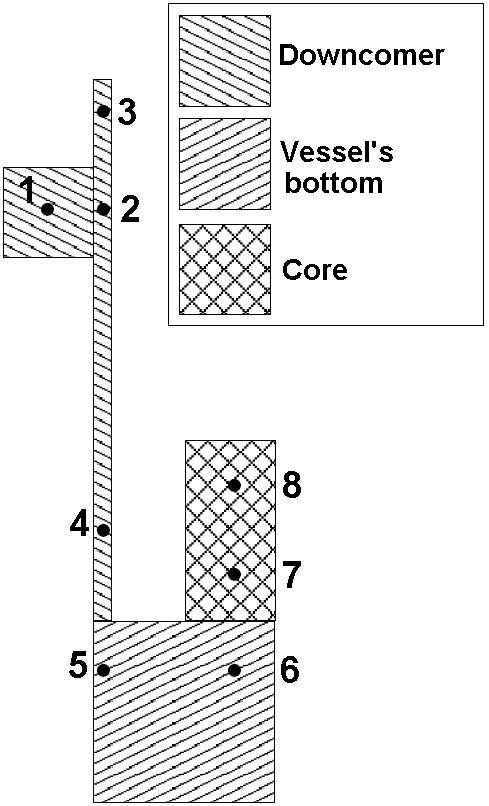
\includegraphics[width=4cm,height=6.8cm]{\repgraphics/fig07.jpg}}}
\parbox{7cm}{%
\begin{center}
\begin{tabular}{|c|c|c|c|}
\hline
Points & X(m) & Y(m) & Z(m)\\
\hline
1 & -0.25 & 2.25 & 0 \\
\hline
2 & 0.05 & 2.25 & 0 \\
\hline
3 & 0.05 & 2.75 & 0 \\
\hline
4 & 0.05 & 0.5 & 0 \\
\hline
5 & 0.05 & -0.25 & 0 \\
\hline
6 & 0.75 & -0.25 & 0 \\
\hline
7 & 0.75 & 0.25 & 0 \\
\hline
8 & 0.75 & 0.75 & 0 \\
\hline
\end{tabular}
\end{center}
}
\caption{Position and coordinates of probes in the full domain}
\label{figante25}
\end{figure}

In addition the domain boundary will be post-processed. This allows to check the
boundary conditions, and especially that of the passive scalar. 


	\subsection{Results}
%---------------------------

Figure \ref{fige1_e2} shows the boundary domain colored by the passive
scalar boundary conditions. The different regions of boundary
conditions defined earlier can be checked. 

\begin{figure}[h!]
\begin{center}
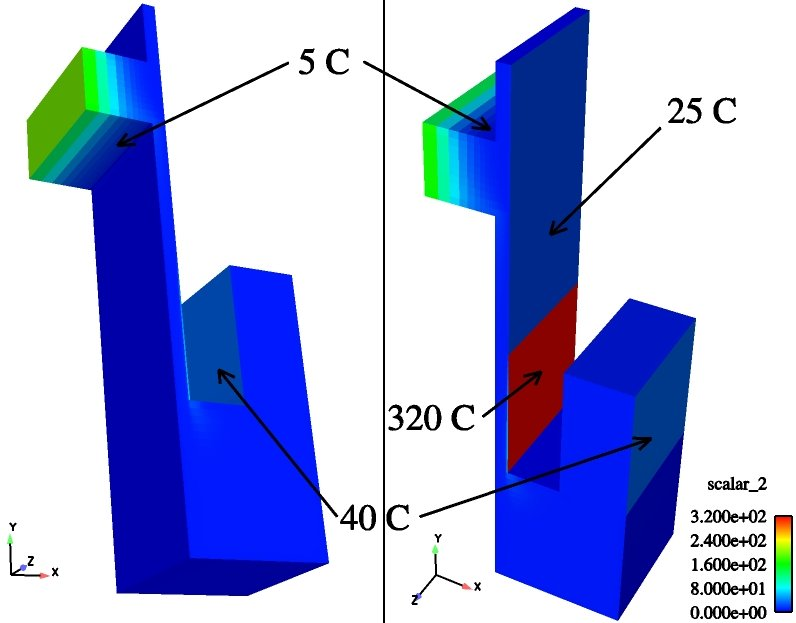
\includegraphics[width=14cm,height=11cm]{\repgraphics/c2_p7.jpg} 
\caption{View of the boundary domain colored by the scalar\_2 variable - Case 2}
\label{fige1_e2}
\end{center}
\end{figure}

Figure \ref{fige2_e2} presents results obtained at different times of the
calculation. They were plotted from the post-processing files, with EnSight.

\begin{figure}
\begin{center}
\begin{tabular}{cc}
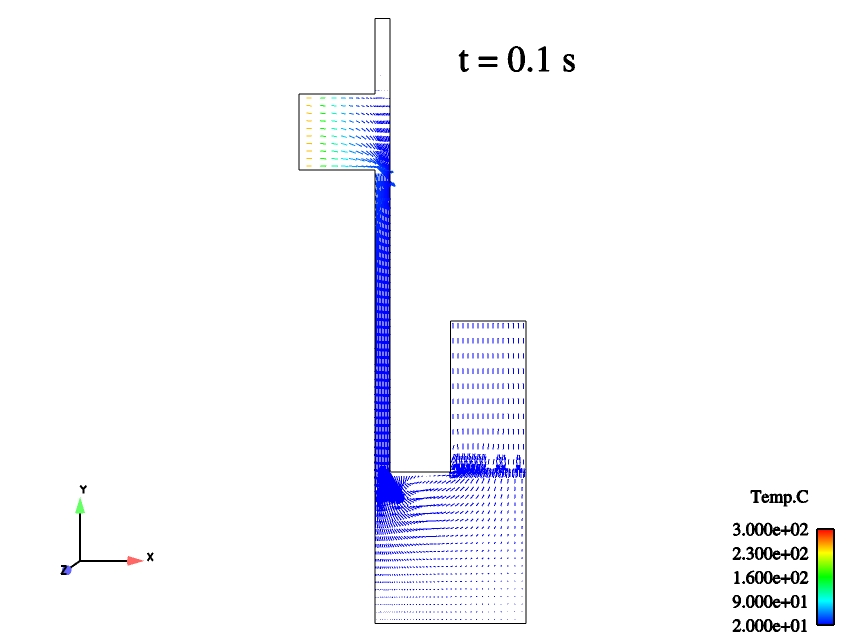
\includegraphics[width=6cm,height=6cm]{\repgraphics/c2_p1.jpg} & 
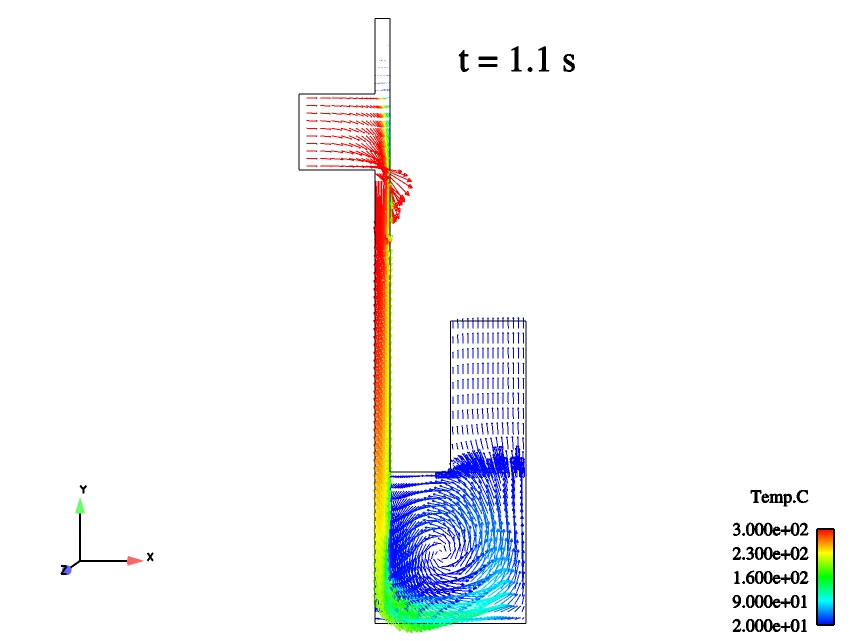
\includegraphics[width=6cm,height=6cm]{\repgraphics/c2_p2.jpg} \\
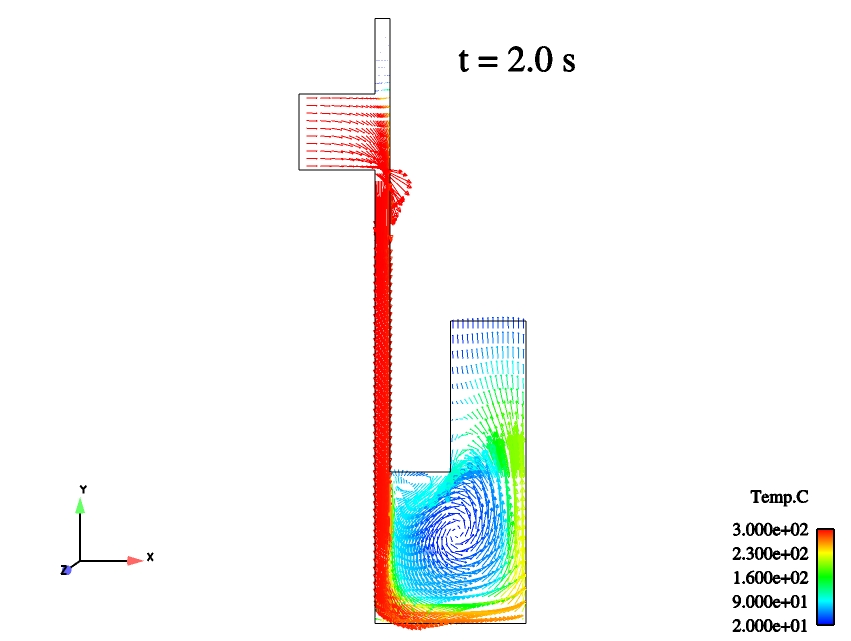
\includegraphics[width=6cm,height=6cm]{\repgraphics/c2_p3.jpg} & 
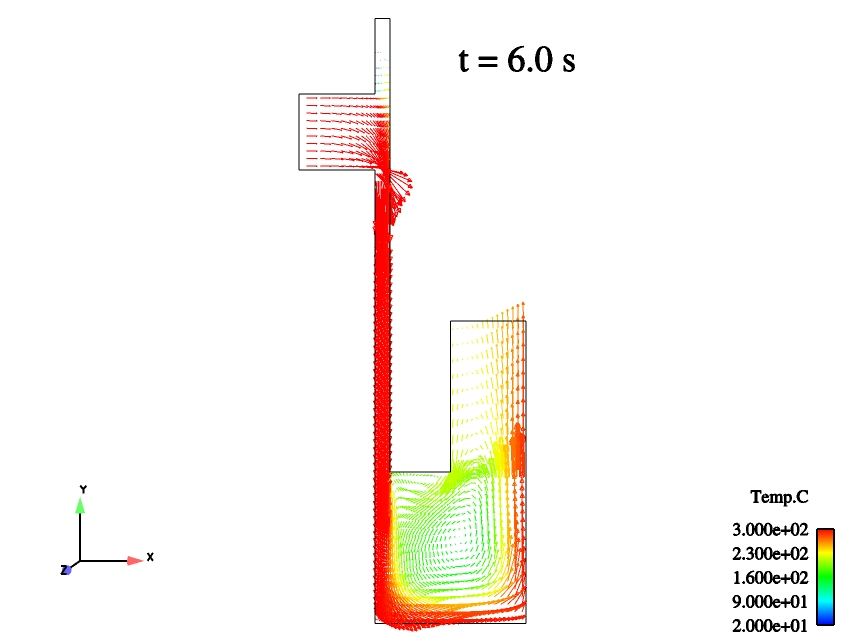
\includegraphics[width=6cm,height=6cm]{\repgraphics/c2_p4.jpg} \\
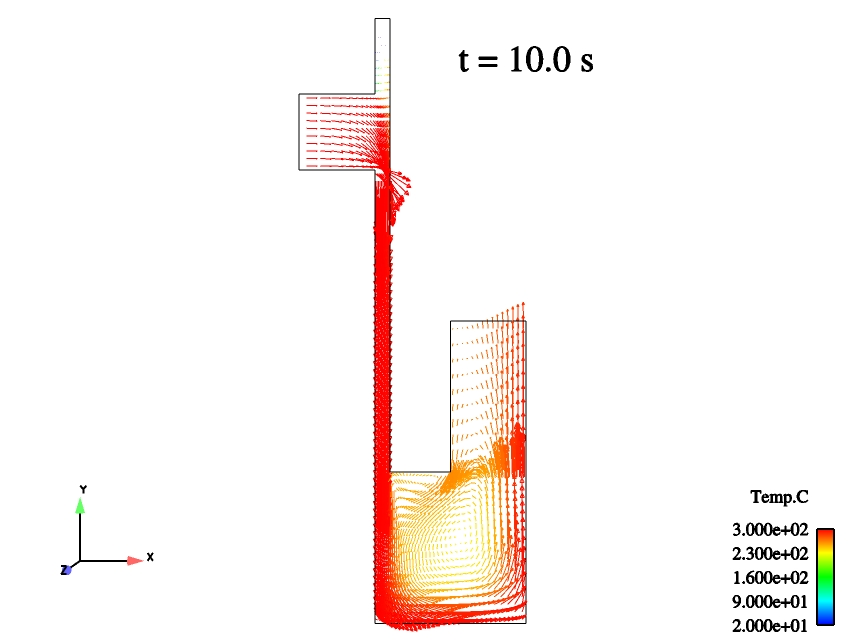
\includegraphics[width=6cm,height=6cm]{\repgraphics/c2_p5.jpg} & 
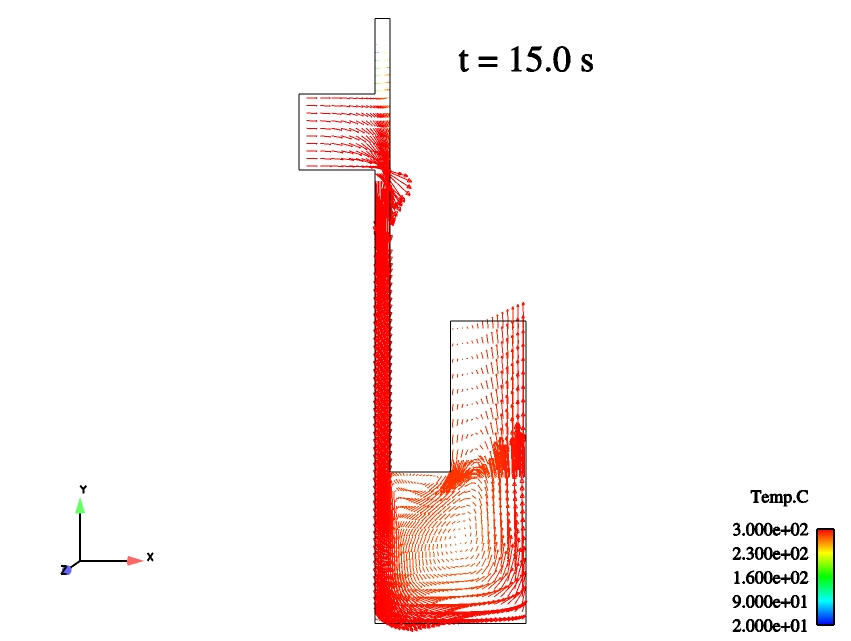
\includegraphics[width=6cm,height=6cm]{\repgraphics/c2_p6.jpg} \\
\end{tabular}
\caption{Water velocity field colored by temperature at different time steps - Case 2}
\label{fige2_e2}
\end{center}
\end{figure}

%                      Code_Saturne version 1.3
%                      ------------------------
%
%     This file is part of the Code_Saturne Kernel, element of the
%     Code_Saturne CFD tool.
%
%     Copyright (C) 1998-2007 EDF S.A., France
%
%     contact: saturne-support@edf.fr
%
%     The Code_Saturne Kernel is free software; you can redistribute it
%     and/or modify it under the terms of the GNU General Public License
%     as published by the Free Software Foundation; either version 2 of
%     the License, or (at your option) any later version.
%
%     The Code_Saturne Kernel is distributed in the hope that it will be
%     useful, but WITHOUT ANY WARRANTY; without even the implied warranty
%     of MERCHANTABILITY or FITNESS FOR A PARTICULAR PURPOSE.  See the
%     GNU General Public License for more details.
%
%     You should have received a copy of the GNU General Public License
%     along with the Code_Saturne Kernel; if not, write to the
%     Free Software Foundation, Inc.,
%     51 Franklin St, Fifth Floor,
%     Boston, MA  02110-1301  USA
%
%-----------------------------------------------------------------------
\newpage
%-----------------------------------------------------------------------------------------------------------------
\section{CASE 3:  Time dependent boundary conditions and variable fluid density}
%-----------------------------------------------------------------------------------------------------------------
In this case some boundary conditions will be time dependent and some physycal
characteristics of the fluid will be dependent on the temperature.

        \subsection{Calculation options}
%-----------------------------------------

The options for this case are the same as in case 2, except for the variable fluid density:
\begin{itemize}
\renewcommand{\labelitemi}{$\rightarrow$}
        \item Flow type: unsteady flow
        \item Time step: uniform and constant
        \item Turbulence model: $k-\epsilon$
        \item Scalar(s): 1 - temperature\\
      \hspace*{1.6cm} 2 - passive scalar
        \item Physical properties: uniform and constant (except density)
        \item Management of monitoring points
\end{itemize}


        \subsection{Initial and boundary conditions}
%---------------------------------------------------

\begin{itemize}
\renewcommand{\labelitemi}{$\rightarrow$}
        \item Initialization: 20\degresC\ for temperature (default value) \\
        \hspace*{2.1cm}        10 for the passive scalar
\end{itemize}

The boundary conditions are defined in the user interface and depend on the
boundary zone. The time dependence of the temperature boundary condition implies
the use of a Fortran user routine (see below).

\begin{itemize}
        \item {\bfseries Flow inlet}: Dirichlet condition, an inlet velocity of
$1\ m.s^{-1}$, a time dependent inlet temperature and a value of 200 for the
passive scalar are imposed
        \item {\bfseries Outlet}: default value
        \item {\bfseries Walls}: velocity, pressure and thermal scalar: default value \\
                    \hspace*{1.25cm} passive scalar: different conditions
depending on the color and geometric parameters
\end{itemize}

The boundary conditions for the passive scalar are identical as in case 2,
as specified in the following table:

\begin{center}
\begin{tabular}{|c|c|c|}
\hline
Wall & Nature & Value \\
\hline
wall\_1 & Dirichlet  & 0 \\
\hline
wall\_2 & Dirichlet  & 5 \\
\hline
wall\_3 & Dirichlet  & 0 \\
\hline
wall\_4 & Dirichlet  & 25 \\
\hline
wall\_5 & Dirichlet  & 320 \\
\hline
wall\_6 & Dirichlet  & 40 \\
\hline
\end{tabular}
\end{center}

The ``wall\_1'' to ``wall\_6'' regions are defined as follows, through color
references and geometric localization:
\begin{center}
\begin{tabular}{c|c}
Label & Color and geometric parameters \\
\hline
wall\_1 & 24 and $0.1\leqslant X$ and $X\leqslant 0.5$ \\
wall\_2 & 2 or 3 \\
wall\_3 & 4 or 7 or 21 or 22 or 23 \\
wall\_4 & 6 and $Y>1$ \\
wall\_5 & 6 and $Y\leqslant1$ \\
wall\_6 & 31 or 33 \\
\end{tabular}
\end{center}

Figure \ref{figante23} shows the colors used for boundary conditions and
table \ref{tabante31} defines the correspondance between the colors and
the type of boundary condition to use.

\begin{table}[htp]
\begin{center}
\begin{tabular}{|c|c|}
\hline
Colors & Conditions \\
\hline
1 & Inlet \\
\hline
34 & Outlet \\
\hline
2 3 4 6 7 21 22 23 31 33 & Wall \\
\hline
24 for $0.1 \leq X \leq 0.5$ & Wall \\
\hline
8 9 28 29 38 39 & Symmetry \\
\hline
\end{tabular}
\caption{Boundary faces colors and associated references}
\label{tabante31}
\end{center}
\end{table}


        \subsection{Parameters}
%------------------------------

All the parameter necessary to this study can be defined through the Graphical
Interface, except the time dependent boundary conditions and the variable
density that have to be specified in user routines.

\begin{center}
\begin{tabular}{|l|c|}
\hline
\multicolumn{2}{|c|}{Parameters of calculation control} \\
\hline
Number of iterations & $300$ \\
\hline
Reference time step & $0.05$ \\
\hline
Output period for post-processing files& $2$ \\
\hline
\end{tabular}\\
\end{center}

In order to paste the separate meshes into a single domain, colors 5, 24 and 32
will have to be pasted through the Graphical Interface.


        \subsection{User routines}
%---------------------------------

The following routines have to be copied from the folder FORT/USER/base into the
folder FORT\footnote{only when they appear in the FORT directory will they be
taken into account by the code}: usclim.F and usphyv.F.

$\bullet$ {\bfseries usclim.F}\\
This routine allows to define advanced boundary conditions on the boundary
faces. Even if usclim.F is used, all boundary conditions have to be defined in
the Graphical User Interface. Only the conditions that differ from this first
definition need appear in usclim.F. The boundary conditions defined in usclim.F
will replace those specified in the Graphical Interface.

In this case, the temperature at entry is supposed variable in time, following
the law:
\begin{equation}
\left\{\begin{array}{ll}
T = 20 + 100t & \text{for }0\leqslant t \leqslant 3.8\\
T = 400 & \text{for } t > 3.8
\end{array}\right.
\end{equation}
where $T$ is the temperature in \degresC\ and $t$ is the time in $s$.


\begin{figure}[h!]
\begin{center}
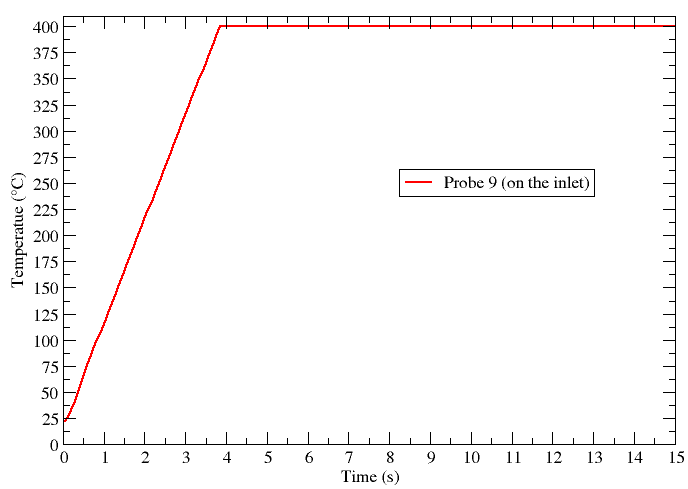
\includegraphics[width=9cm,height=6.4cm]{\repgraphics/probe9.png}
\caption{Time evolution of the temperature at inlet}
\label{figp9_e3}
\end{center}
\end{figure}


$\bullet$ {\bfseries usphyv.F}\\
This routine allows to specify variable physical properties, density in
particular. In this case, the variation law given as an example in the routine
will be appropriate:
\begin{equation}
\rho = T.(A.T + B) + C
\end{equation}
where $\rho$ is the density, $T$ is the temperature, $A = -4.0668\times10^{-3}$,
$B =-5.0754\times 10^{-2}$ and $C = 1\,000.9$

\textbf{Note:} in the example routine, the example is protected by a test to prevent any
undesired use. Do not forget to deactivate it.

In order for the variable density to have an effect on the flow, gravity must be
set to a non-zero value. $\vect{g} = -9.81 \vect{e}_y$ will be specified in the
Graphical Interface.

        \subsection{Output management}
%-------------------------------------

The output management is the same as in case 2, except that a nineth monitoring
point will be added, just at the entry, to monitor the temperature evolution at inlet.

\begin{figure}[htp]
\parbox{8cm}{%
\centerline{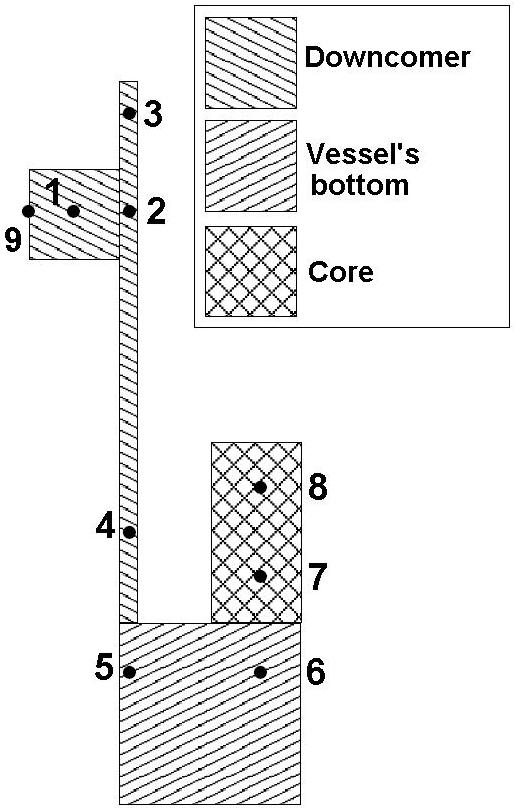
\includegraphics[width=4cm,height=6.8cm]{\repgraphics/fig08.jpg}}}
\parbox{7cm}{%
\begin{center}
\begin{tabular}{|c|c|c|c|}
\hline
Points & X(m) & Y(m) & Z(m)\\
\hline
1 & -0.25 & 2.25 & 0 \\
\hline
2 & 0.05 & 2.25 & 0 \\
\hline
3 & 0.05 & 2.75 & 0 \\
\hline
4 & 0.05 & 0.5 & 0 \\
\hline
5 & 0.05 & -0.25 & 0 \\
\hline
6 & 0.75 & -0.25 & 0 \\
\hline
7 & 0.75 & 0.25 & 0 \\
\hline
8 & 0.75 & 0.75 & 0 \\
\hline
9 & -0.5 & 2.25 & 0 \\
\hline
\end{tabular}
\end{center}
}
\caption{Position and coordinates of probes in the full domain}
\label{figante32}
\end{figure}

In this case, the {\itshape Pressure}, the {\itshape Tubulent energy} and the
{\itshape Dissipation} will be removed from the listing file.

The {\itshape Courant number} (CFL) and {\itshape Fourier number} will be
removed from the
post-processing results\footnote{this can be very useful to save some disk space
if some variables are of no interest, as post-processing files can be large}.

Eventually, probes will be defined for chronological records, folowing the data
given in figure \ref{figante25}. Then the {\itshape total pressure} will be
deactivated from all probes and the {\itshape Velocity U} will be only activated
on probes  1, 2, 6, 7 and 8.


In addition the domain boundary will be post-processed. This allows to check the
boundary conditions, and especially that of the temperature and passive scalar.


        \subsection{Calculation restart}
%---------------------------------------

After the first run, the calculation will be continued for another 400 time
steps. The calculation restart is managed through the Graphical Interface.


        \subsection{Results}
%---------------------------
Figure \ref{fige3_e3} shows the time evolution of temperature recorded on each
monitoring probe.
\begin{figure}[hb]
\begin{center}
\begin{tabular}{cc}
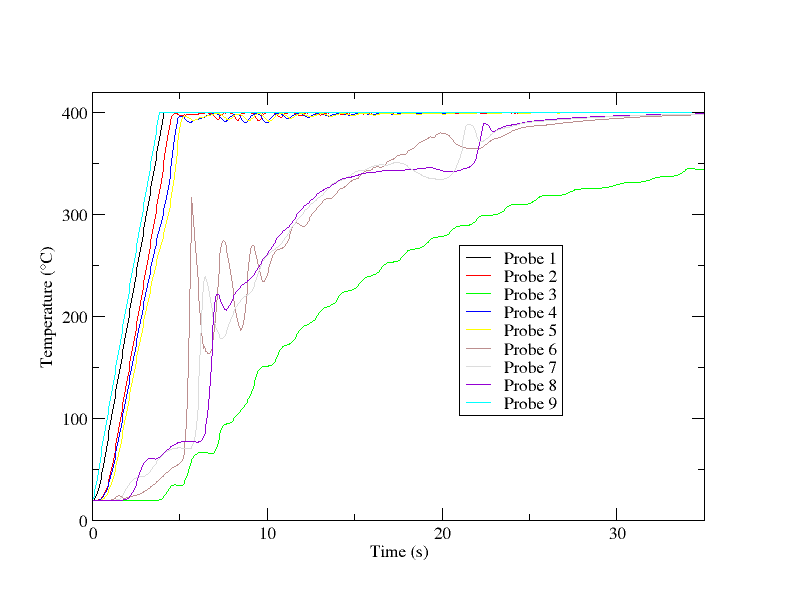
\includegraphics[width=11cm]{\repgraphics/evotemp_case3.png} \\
\end{tabular}
\caption{Time evolution of temperature at monitoring probes for case 3}
\label{fige3_e3}
\end{center}
\end{figure}

Figure \ref{fige1_e3} shows the velocity fields colored by temperature in the
first run of calculation. Figure \ref{fige2_e3} shows the velocity fields in the
second calculation (restart of the first one).

\begin{figure}
\begin{center}
\begin{tabular}{cc}
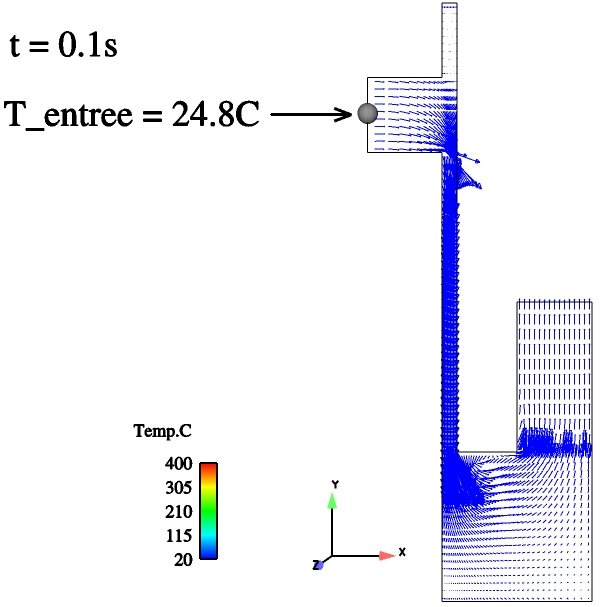
\includegraphics[height=6cm]{\repgraphics/case3_p1.jpg} &
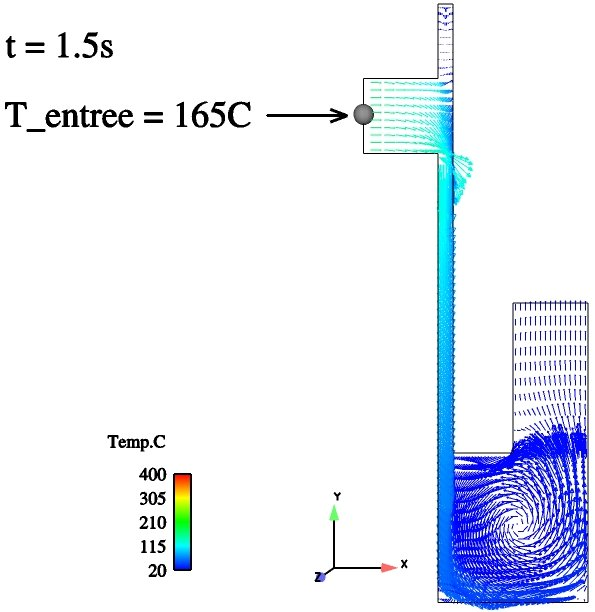
\includegraphics[height=6cm]{\repgraphics/case3_p2.jpg} \\
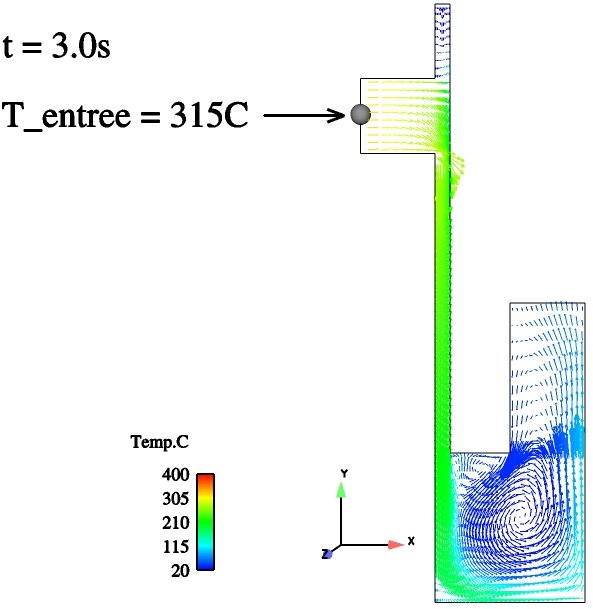
\includegraphics[height=6cm]{\repgraphics/case3_p3.jpg} &
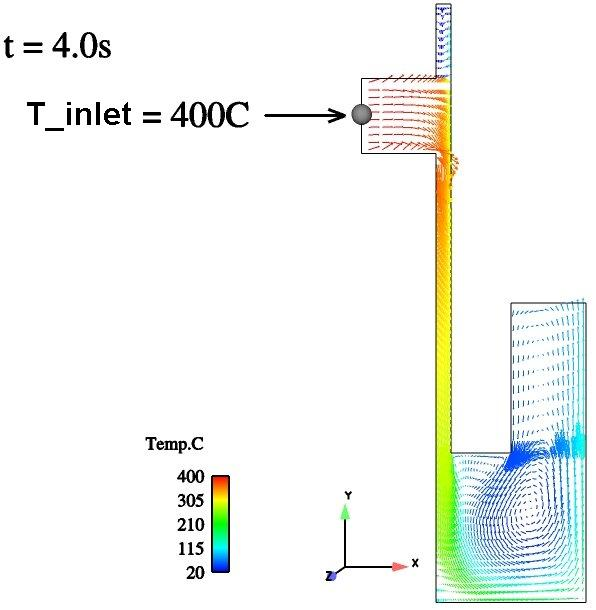
\includegraphics[height=6cm]{\repgraphics/case3_p4.jpg} \\
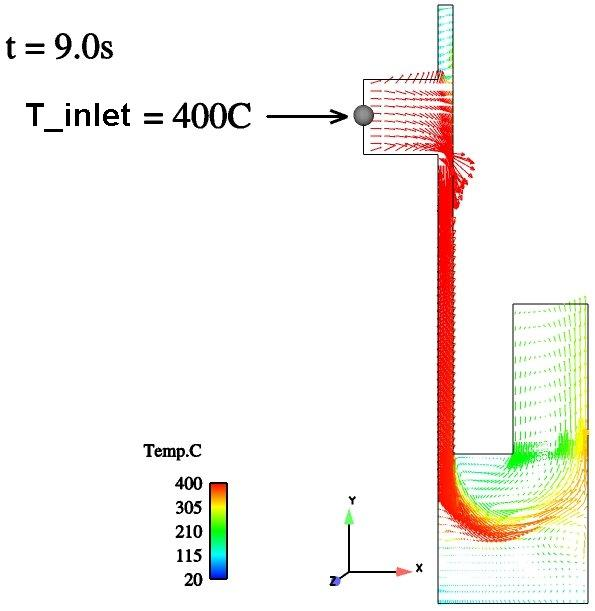
\includegraphics[height=6cm]{\repgraphics/case3_p5.jpg} &
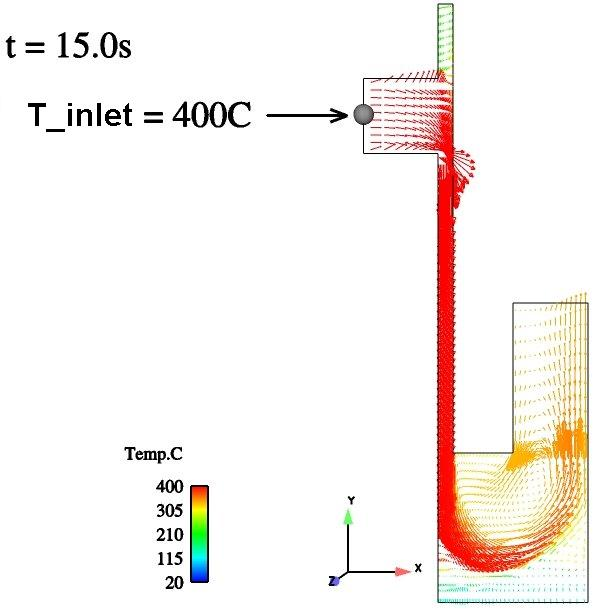
\includegraphics[height=6cm]{\repgraphics/case3_p6.jpg} \\
\end{tabular}
\caption{Water velocity field colored by temperature and inlet temperature value
at different time steps (first calculation)}
\label{fige1_e3}
\end{center}
\end{figure}


\begin{figure}
\begin{center}
\begin{tabular}{cc}
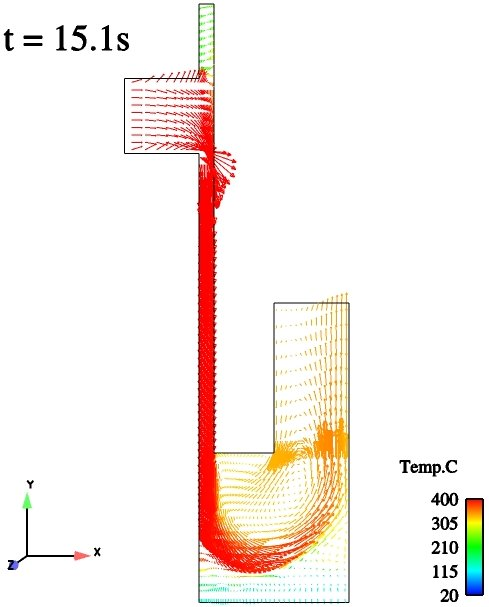
\includegraphics[height=7.5cm]{\repgraphics/case3_p7.jpg} &
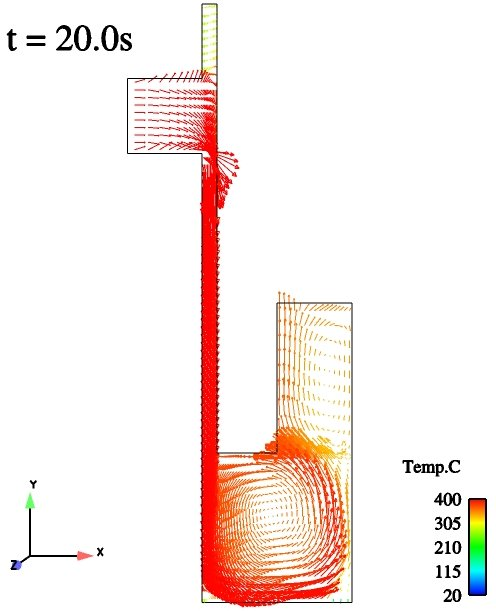
\includegraphics[height=7.5cm]{\repgraphics/case3_p8.jpg} \\
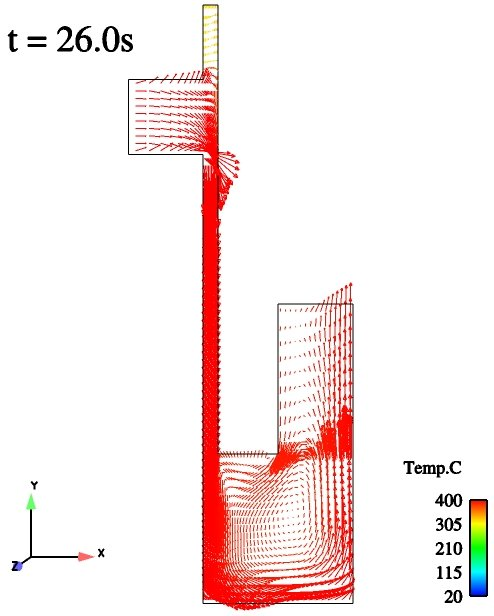
\includegraphics[height=7.5cm]{\repgraphics/case3_p9.jpg} &
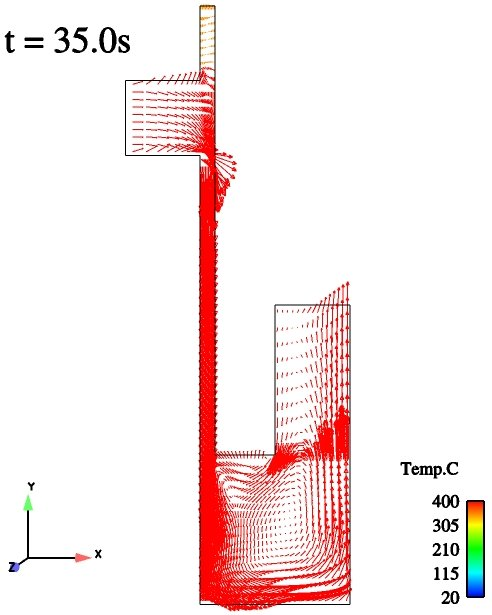
\includegraphics[height=7.5cm]{\repgraphics/case3_p10.jpg} \\
\end{tabular}
\caption{Water velocity field colored by temperature and inlet temperature value
at different time steps (second calculation)}
\label{fige2_e3}
\end{center}
\end{figure}







%                      Code_Saturne version 1.3
%                      ------------------------
%
%     This file is part of the Code_Saturne Kernel, element of the
%     Code_Saturne CFD tool.
%
%     Copyright (C) 1998-2008 EDF S.A., France
%
%     contact: saturne-support@edf.fr
%
%     The Code_Saturne Kernel is free software; you can redistribute it
%     and/or modify it under the terms of the GNU General Public License
%     as published by the Free Software Foundation; either version 2 of
%     the License, or (at your option) any later version.
%
%     The Code_Saturne Kernel is distributed in the hope that it will be
%     useful, but WITHOUT ANY WARRANTY; without even the implied warranty
%     of MERCHANTABILITY or FITNESS FOR A PARTICULAR PURPOSE.  See the
%     GNU General Public License for more details.
%
%     You should have received a copy of the GNU General Public License
%     along with the Code_Saturne Kernel; if not, write to the
%     Free Software Foundation, Inc.,
%     51 Franklin St, Fifth Floor,
%     Boston, MA  02110-1301  USA
%
%-----------------------------------------------------------------------
\newpage
%-------------------------------------------------------------
\section{CASE 4: Head loss, parallelism and spatial average}
%-------------------------------------------------------------
\label{prg_case4}%
This case will be run in parallel on two processors. Head loss will be used to
simulate the presence of an obstacle in the flow and the spatial average of the
temperature will be calculated at each time step.

        \subsection{Calculation options}
%-----------------------------------------

The options for this case are the same as in case 3:
\begin{itemize}
\renewcommand{\labelitemi}{$\rightarrow$}
        \item Flow type: unsteady flow
        \item Time step: uniform and constant
        \item Turbulence model: $k-\epsilon$
        \item Scalar(s): 1 - temperature\\
      \hspace*{1.6cm} 2 - passive scalar
        \item Physical properties: uniform and constant (except density)
        \item Management of monitoring points
\end{itemize}


        \subsection{Initial and boundary conditions}
%---------------------------------------------------

\begin{itemize}
\renewcommand{\labelitemi}{$\rightarrow$}
        \item Initialization: 20\degresC\ for temperature (default value) \\
        \hspace*{2.1cm}        10 for the passive scalar
\end{itemize}

The boundary conditions are defined in the user interface and depend on the
boundary zone.

\begin{itemize}
        \item {\bfseries Flow inlet}: Dirichlet condition, an inlet velocity of
$1\ m.s^{-1}$ and a time dependent inlet temperature are imposed
        \item {\bfseries Outlet}: default value
        \item {\bfseries Walls}: velocity, pressure and thermal scalar: default value \\
                    \hspace*{1.25cm} passive scalar: different conditions
depending on the color and geometric parameters
\end{itemize}

The boundary conditions for the passive scalar are identical as in case 2,
as specified in the following table:

\begin{center}
\begin{tabular}{|c|c|c|}
\hline
Wall & Nature & Value \\
\hline
wall\_1 & Dirichlet  & 0 \\
\hline
wall\_2 & Dirichlet  & 5 \\
\hline
wall\_3 & Dirichlet  & 0 \\
\hline
wall\_4 & Dirichlet  & 25 \\
\hline
wall\_5 & Dirichlet  & 320 \\
\hline
wall\_6 & Dirichlet  & 40 \\
\hline
\end{tabular}
\end{center}

The ``wall\_1'' to ``wall\_6'' regions are defined as follows, through color
references and geometric localization:
\begin{center}
\begin{tabular}{c|c}
Label & Color and geometric parameters \\
\hline
wall\_1 & 24 and $0.1\leqslant X$ and $X\leqslant 0.5$ \\
wall\_2 & 2 or 3 \\
wall\_3 & 4 or 7 or 21 or 22 or 23 \\
wall\_4 & 6 and $Y>1$ \\
wall\_5 & 6 and $Y\leqslant1$ \\
wall\_6 & 31 or 33 \\
\end{tabular}
\end{center}

Figure \ref{figante23} shows the colors used for boundary conditions and
table \ref{tabante41} defines the correspondance between the colors and
the type of boundary condition to use.

\begin{table}[htp]
\begin{center}
\begin{tabular}{|c|c|}
\hline
Colors & Conditions \\
\hline
1 & Inlet \\
\hline
34 & Outlet \\
\hline
2 3 4 6 7 21 22 23 31 33 & Wall \\
\hline
24 for $0.1 \leq X \leq 0.5$ & Wall \\
\hline
8 9 28 29 38 39 & Symmetry \\
\hline
\end{tabular}
\caption{Boundary faces colors and associated references}
\label{tabante41}
\end{center}
\end{table}



        \subsection{Head loss}
%-----------------------------

To simulate the presence of an obstacle $0.20\ m$ large and $0.5\ m$ high in the
vessel, a zone of head loss will be created in the domain (fig \ref{figante41}).
The head loss zone is situated between the coordinates $X=0.2\ m$ and $X=0.4\ m$,
and $Y=-0.75\ m$ and $Y=-0.25\ m$. The head loss coefficient to apply is $10^4$
and is isotropic.

\begin{figure}[h!]
\begin{center}
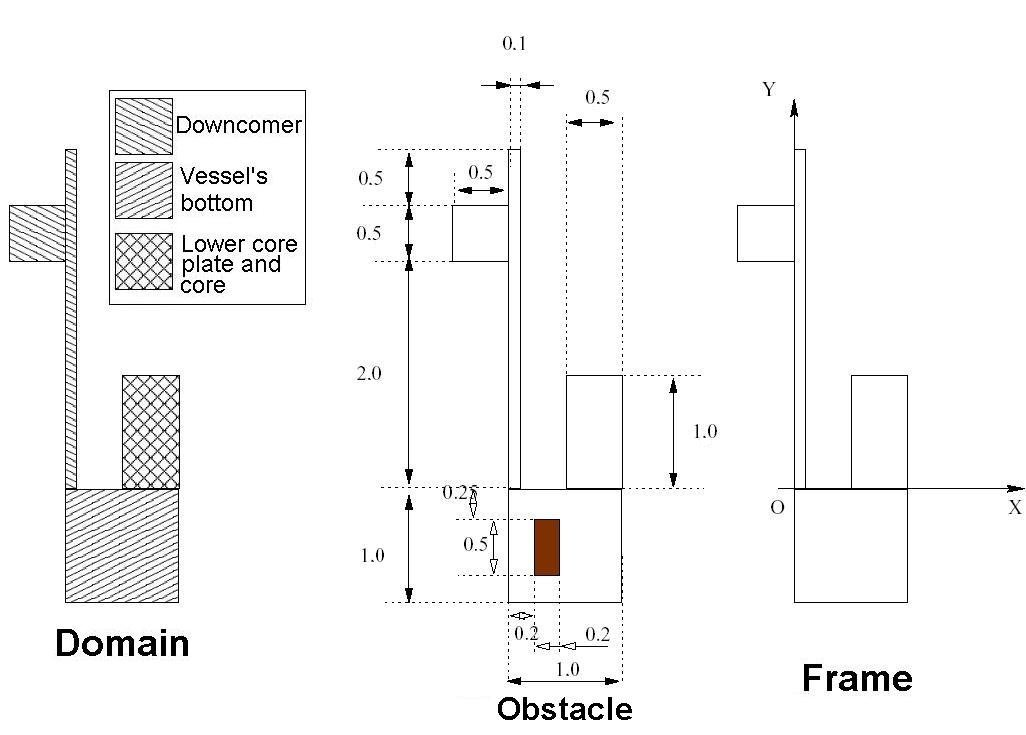
\includegraphics[width=10cm,height=8cm]{\repgraphics/fig09.jpg}
\caption{Full domain geometry with the obstacle}
\label{figante41}
\end{center}
\end{figure}



        \subsection{Parameters}
%------------------------------

All the parameter necessary to this study can be defined through the Graphical
Interface, except the time dependent boundary conditions, the variable
density and the head loss that have to be specified in user routines. The
calculation of the spatial average is also defined by a user routine.


\begin{center}
\begin{tabular}{|l|c|}
\hline
\multicolumn{2}{|c|}{Parameters of calculation control} \\
\hline
Number of iterations & $300$ \\
\hline
Reference time step & $0.05$ \\
\hline
Output period for post-processing files& $2$ \\
\hline
The calculation will be run in parallel on 2 processors \\
\end{tabular}\\
\end{center}

In order to paste the separate meshes into a single domain, colors 5, 24 and 32
will have to be pasted through the Graphical Interface.


        \subsection{User routines}
%---------------------------------

The following routines have to be copied from the folder FORT/USER/base into the
folder FORT\footnote{only when they appear in the FORT directory will they be
taken into account by the code}: usclim.F, usphyv.F, usproj.F and uskpdc.F.

$\bullet$ {\bfseries usclim.F}\\
This routine allows to define advanced boundary conditions on the boundary
faces. Even if usclim.F is used, all boundary conditions have to be defined in
the Graphical User Interface. Only the conditions that differ from this first
definition need appear in usclim.F. The boundary conditions defined in usclim.F
will replace those specified in the Graphical Interface.

In this case, the temperature at entry is supposed variable in time, following
the law:
\begin{equation}
\left\{\begin{array}{ll}
T = 20 + 100t & \text{for }0\leqslant t \leqslant 3.8\\
T = 400 & \text{for } t > 3.8
\end{array}\right.
\end{equation}
where $T$ is the temperature in \degresC\ and $t$ is the time in $s$.


\begin{figure}[h!]
\begin{center}
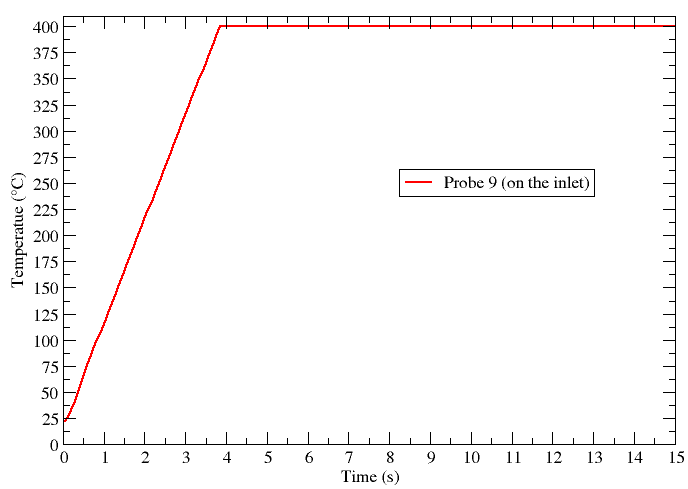
\includegraphics[width=9cm,height=6.4cm]{\repgraphics/probe9.png}
\caption{Time evolution of the temperature at inlet}
\label{figp9_e4}
\end{center}
\end{figure}


$\bullet$ {\bfseries usphyv.F}\\
This routine allows to specify variable physical properties, density in
particular. In this case, the variation law given as an example in the routine
will be appropriate:
\begin{equation}
\rho = T.(A.T + B) + C
\end{equation}
where $\rho$ is the density, $T$ is the temperature, $A = -4.0668\times10^{-3}$,
$B =-5.0754\times 10^{-2}$ and $C = 1\,000.9$

\textbf{Note:} in the example routine, the example is protected by a test to prevent any
undesired use. Do not forget to deactivate it.

In order for the variable density to have an effect on the flow, gravity must be
set to a non-zero value. $\vect{g} = -9.81 \vect{e}_y$ will be specified in the
Graphical Interface.


$\bullet$ {\bfseries usproj.F}\\
This routine is called at the end of each time step and has access to the whole
set of variables of the code. It is therefore useful for many user-specific
post-processing, including the calculation of a spatial average in the present
case.\\
The spatial average of the temperature will be calculated at each time step and
the result wrote in a file named ``moy.dat''. The values are saved in order
to draw the time evolution of the average temperature.

Beware when calculating the average. Since the calculation is running in
parallel, computing the sum of the temperatures on ``all the cells'' will only
yield for each processor the sum on the cells managed by this processor. In
order to obtain the full sum, the parallelism routine PARSOM must be used (see
example).

\textbf{Note:} usproj.F contains many examples. They should be removed before
running the case.


$\bullet$ {\bfseries uskpdc.F}

This routine allows to apply head loss on the fluid domain.

The localization of the obstacle is made geometrically, using the
coordinates of the centers of the cells.


If $XYZCEN(1,IEL) \leq 0.40$ and $XYZCEN(1,IEL) \geq 0.20$ \\
and $XYZCEN(2,IEL) \geq -0.75$ and $XYZCEN(2,IEL) \leq -0.25$\\
then an isotropic head loss coefficient $K = 10^{4}$ is applied:\\

$NCKPDP = 3$: the head loss tensor is diagonal \\
$CKUPDC(IELPDC,1) = K*ABS(RTPA(IEL,IU(IPHAS)))$ \\
$CKUPDC(IELPDC,2) = K*ABS(RTPA(IEL,IV(IPHAS)))$ \\
$CKUPDC(IELPDC,3) = K*ABS(RTPA(IEL,IW(IPHAS)))$

        \subsection{Output management}
%-------------------------------------

The output management is the same as in case 3.

\begin{figure}[htp]
\parbox{8cm}{%
\centerline{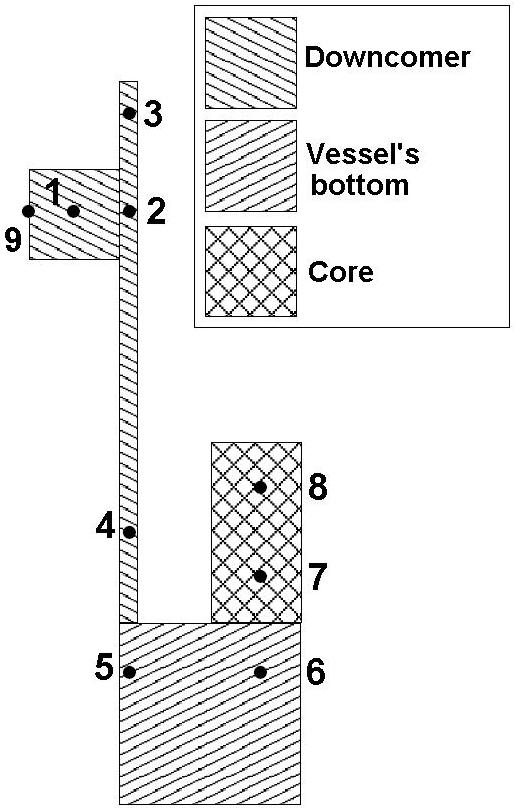
\includegraphics[width=4cm,height=6.8cm]{\repgraphics/fig08.jpg}}}
\parbox{7cm}{%
\begin{center}
\begin{tabular}{|c|c|c|c|}
\hline
Points & X(m) & Y(m) & Z(m)\\
\hline
1 & -0.25 & 2.25 & 0 \\
\hline
2 & 0.05 & 2.25 & 0 \\
\hline
3 & 0.05 & 2.75 & 0 \\
\hline
4 & 0.05 & 0.5 & 0 \\
\hline
5 & 0.05 & -0.25 & 0 \\
\hline
6 & 0.75 & -0.25 & 0 \\
\hline
7 & 0.75 & 0.25 & 0 \\
\hline
8 & 0.75 & 0.75 & 0 \\
\hline
9 & -0.5 & 2.25 & 0 \\
\hline
\end{tabular}
\end{center}
}
\caption{Position and coordinates of probes in the full domain}
\label{figante42}
\end{figure}

In this case, the {\itshape Pressure}, the {\itshape Tubulent energy} and the
{\itshape Dissipation} will be removed from the listing file.

The {\itshape Courant number} (CFL) and {\itshape Fourier number} will be
removed from the
post-processing results\footnote{this can be very useful to save some disk space
if some variables are of no interest, as post-processing files can be large}.

Eventually, probes will be defined for chronological records, folowing the data
given in figure \ref{figante25}. Then the {\itshape total pressure} will be
deactivated from all probes and the {\itshape Velocity U} will be only activated
on probes  1, 2, 6, 7 and 8.


In addition the domain boundary will be post-processed. This allows to check the
boundary conditions, and especially that of the temperature and passive scalar.



        \subsection{Results}
%---------------------------
Figure \ref{fige2_e4} shows the evolution of the spatial average of the temperature.

\begin{figure}[h]
\begin{center}
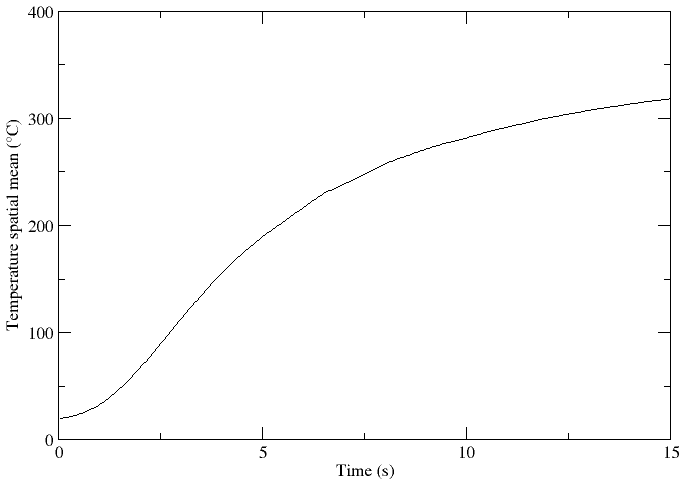
\includegraphics[width=9cm]{\repgraphics/moytemp.png}
\caption{Evolution of spatial average of the temperature as a function of time}
\label{fige2_e4}
\end{center}
\end{figure}

Figure \ref{fige1_e4} shows velocity fields colored by temperature. The effect
of the head loss modeling the obstacle is clearly visible.

\begin{figure}
\begin{center}
\begin{tabular}{cc}
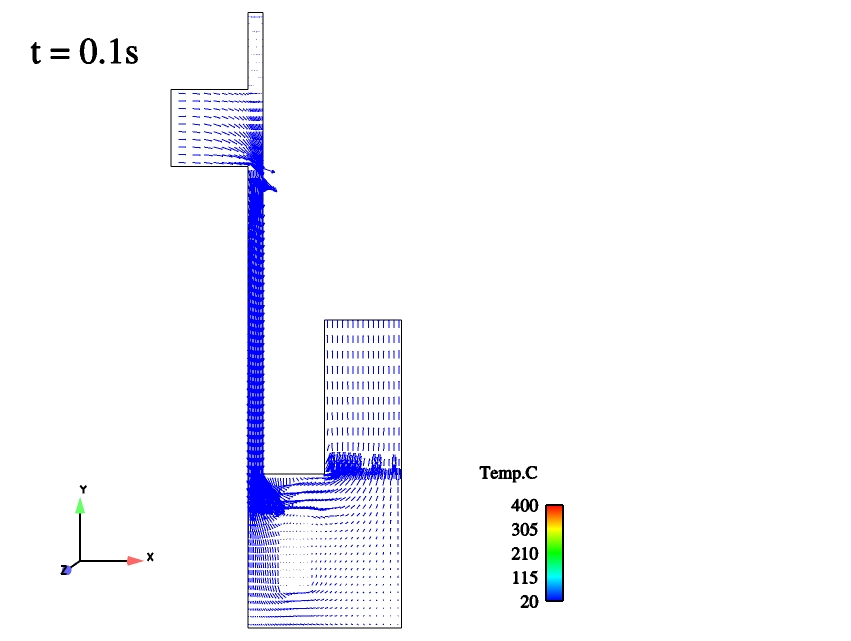
\includegraphics[height=6cm]{\repgraphics/case4_p1.jpg} &
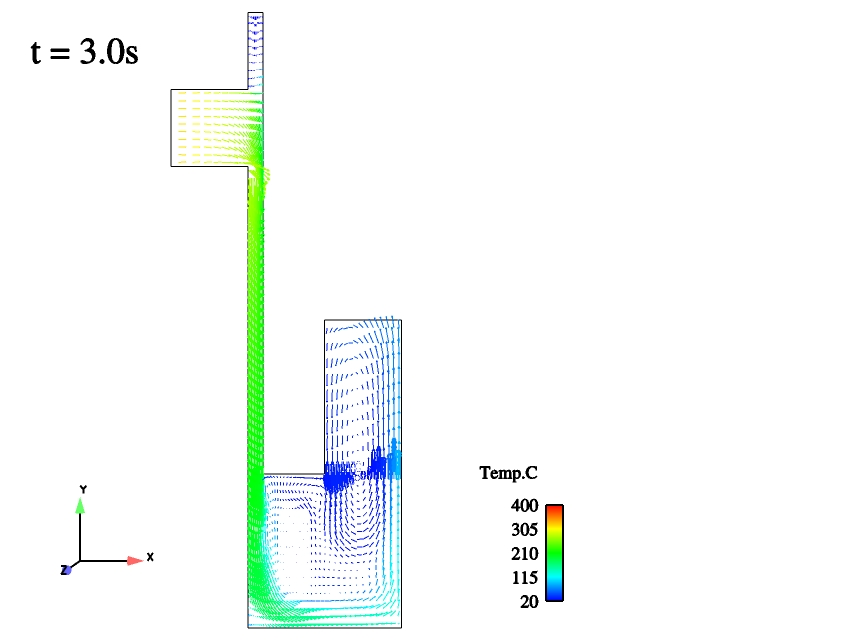
\includegraphics[height=6cm]{\repgraphics/case4_p2.jpg} \\
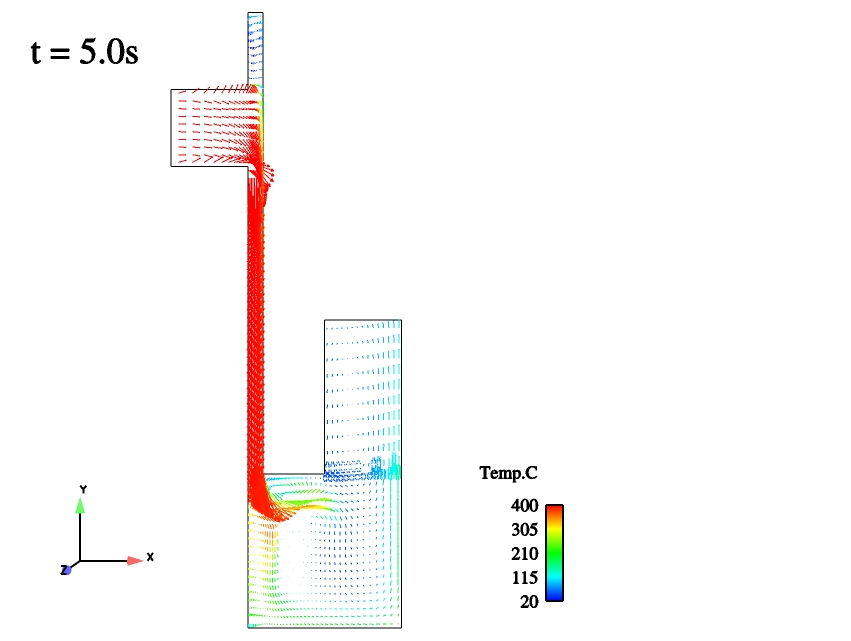
\includegraphics[height=6cm]{\repgraphics/case4_p3.jpg} &
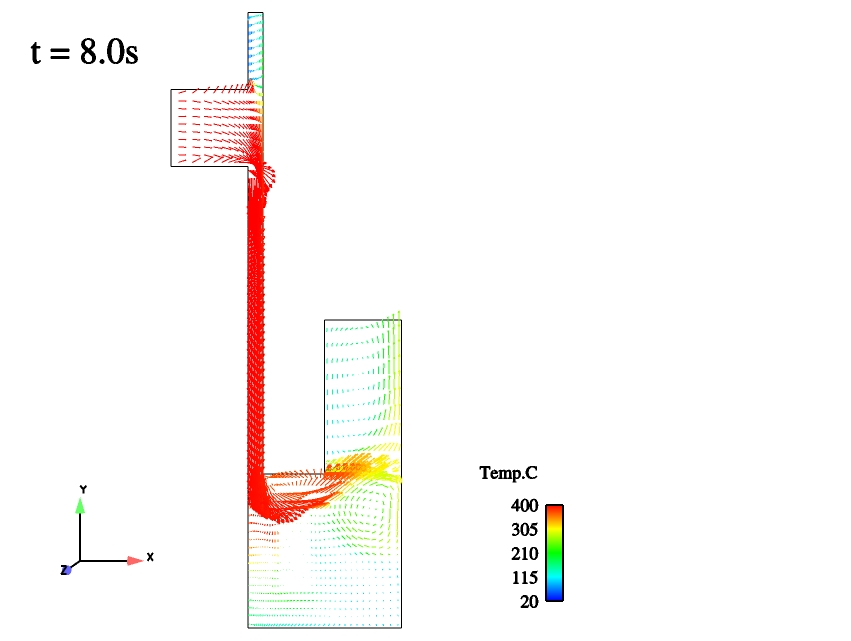
\includegraphics[height=6cm]{\repgraphics/case4_p4.jpg} \\
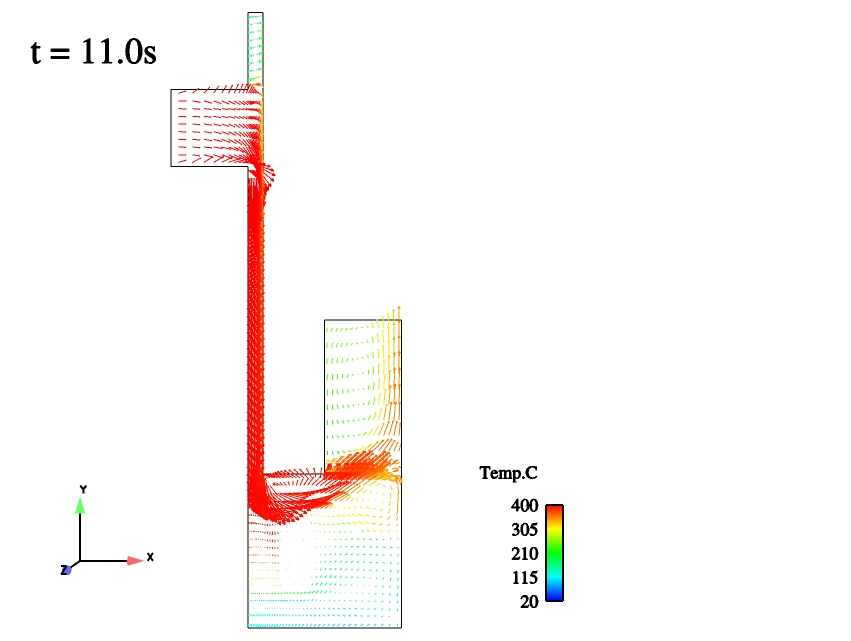
\includegraphics[height=6cm]{\repgraphics/case4_p5.jpg} &
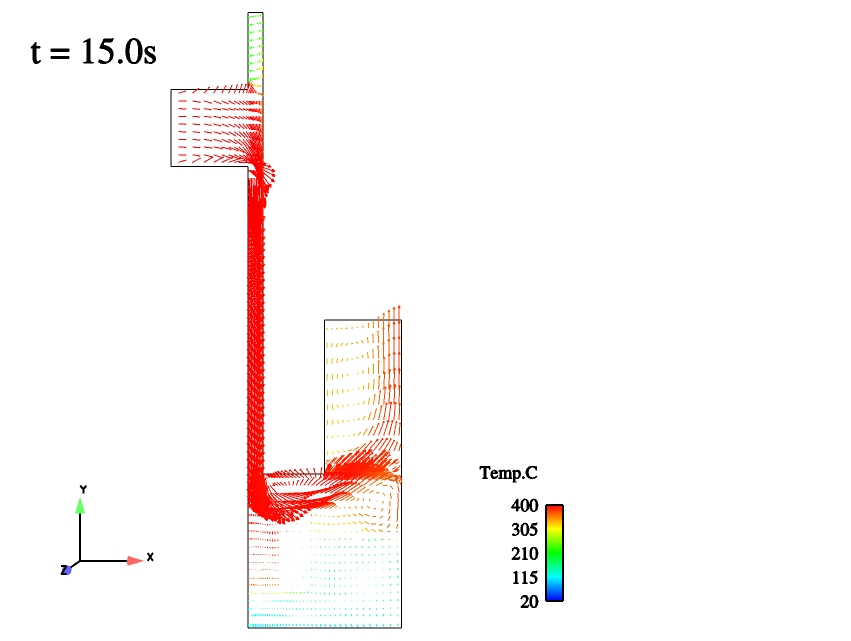
\includegraphics[height=6cm]{\repgraphics/case4_p6.jpg} \\
\end{tabular}
\caption{Water velocity field colored by temperature}
\label{fige1_e4}
\end{center}
\end{figure}



\setcounter{section}{0}
\stepcounter{chapter}
\part{STRATIFIED JUNCTION}
%-----------------------------------------------------------------------
%
%     This file is part of the Code_Saturne Kernel, element of the
%     Code_Saturne CFD tool.
%
%     Copyright (C) 1998-2008 EDF S.A., France
%
%     contact: saturne-support@edf.fr
%
%     The Code_Saturne Kernel is free software; you can redistribute it
%     and/or modify it under the terms of the GNU General Public License
%     as published by the Free Software Foundation; either version 2 of
%     the License, or (at your option) any later version.
%
%     The Code_Saturne Kernel is distributed in the hope that it will be
%     useful, but WITHOUT ANY WARRANTY; without even the implied warranty
%     of MERCHANTABILITY or FITNESS FOR A PARTICULAR PURPOSE.  See the
%     GNU General Public License for more details.
%
%     You should have received a copy of the GNU General Public License
%     along with the Code_Saturne Kernel; if not, write to the
%     Free Software Foundation, Inc.,
%     51 Franklin St, Fifth Floor,
%     Boston, MA  02110-1301  USA
%
%-----------------------------------------------------------------------
\section{General description}
%----------------------------

        \subsection{Objective}
%-----------------------------

The aim of this case is to train the \CS user on a simplified but real 3D
computation. It corresponds to a stratified flow in a T-junction. The test case
will be used to present some advanced post-processing techniques.


        \subsection{Description of the configuration}
%-----------------------------------------------

The configuration is based on a real mock-up designed to characterize thermal
stratification phenomena and associated fluctuations. The geometry is shown on
figure \ref{config}.


\begin{figure}[h!]
\begin{center}
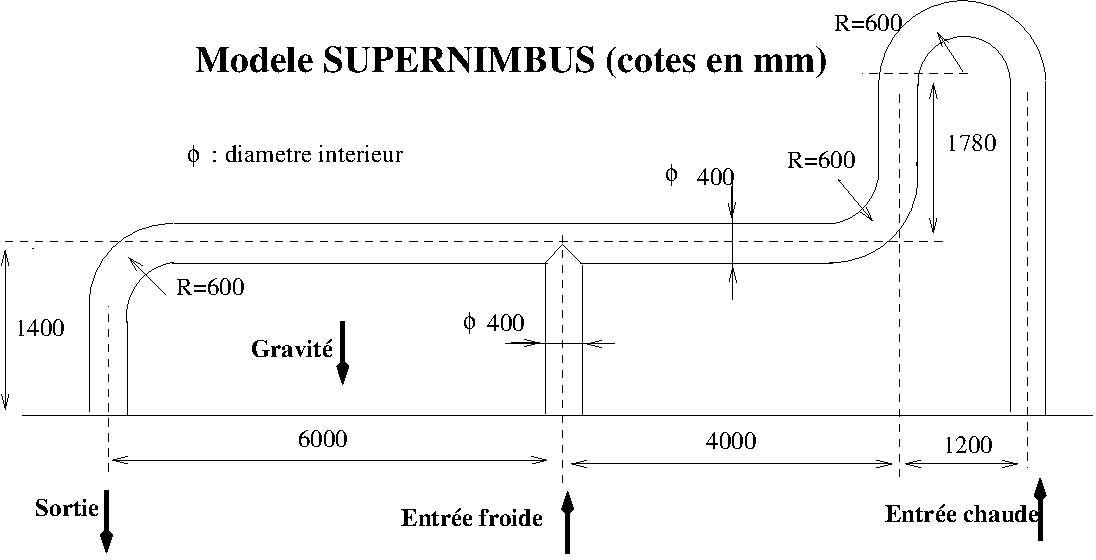
\includegraphics[width=9cm,height=4.5cm]{c5_config}
\caption{Geometry of the case}
\label{config}
\end{center}
\end{figure}

There are two inlets, a hot one in the main pipe and a cold one in the vertical nozzle.
The volumic flow rate is identical in both inlets. It is chosen small enough so that
gravity effects are important with respect to inertia forces. Therefore
cold water creeps backwards from the nozzle towards the elbow until the flow
reaches a stable stratified state.


        \subsection{Characteristics}
%----------------------------------

Characteristics of the geometry: \\

\begin{center}
\begin{tabular}{|l|c|}
\hline
Diameter of the pipe & $D_{b} = 0.40\ m$ \\
\hline
\end{tabular}\\
\end{center}

Characteristics of flow:

\begin{center}
\begin{tabular}{|l|c|}
\hline
Cold branch volume flow rate & $Dv_{cb} = 4\ l.s^{-1}$ \\
\hline
Hot branch volume flow rate & $Dv_{hb} = 4\ l.s^{-1}$ \\
\hline
Cold branch temperature & $T_{cb} = 18.26$\degresC \\
\hline
Hot branch temperature & $T_{hb} = 38.5$\degresC \\
\hline
\end{tabular}\\
\end{center}

The initial water temperature in the domain is equal to 38.5\degresC.

Water specific heat and thermal conductivity are considered constant and
calculated at 18.26\degresC\ and $10^{5}\ Pa$:
\begin{itemize}
        \item heat capacity: $C_{p} = 4_,182.88\ J.kg^{-1}.\mbox{\degresC}^{-1}$
        \item thermal conductivity: $\lambda = 0.601498\ W.m^{-1}.\mbox{\degresC}^{-1}$
\end{itemize}

The water density and dynamic viscosity are variable with the temperature. The
functions are given below.


        \subsection{Mesh characteristics}
%---------------------------------------
The mesh used in the actual study had 125\,000 elements. It has been coarsened
for this example in order for calculations to run faster. The mesh used here
contains 16\,320 elements.

{\bfseries Type}: unstructured mesh

{\bfseries Coordinates system}: cartesian, origin on the middle of the horizontal pipe at the intersection with the nozzle.

{\bfseries Mesh generator used}: SIMAIL

{\bfseries Color definition}: see figure \ref{fige1_e5}.

\begin{figure}[h!]
\begin{center}
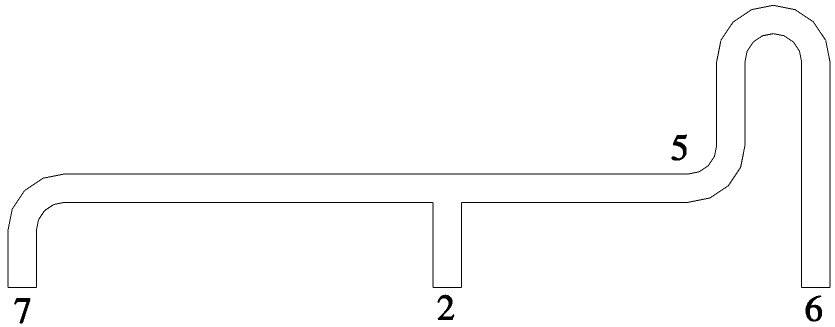
\includegraphics[width=10cm]{color_Snimbus}
\caption{Colors of the boundary faces}
\label{fige1_e5}
\end{center}
\end{figure}


%-----------------------------
\section{CASE 5: Stratified junction}
%-----------------------------
In this case, advanced post-processing features will be used. A specific
pos-processing sub-mesh will be created, containing all the cells with a
temperature lower than 21\degresC, so that it can be visualized (with EnSight
for instance). The variable ``temperature'' will be post-processed on this
sub-mesh. A 2D clip plane will also be extracted along the symmetry plane of the
domain and temperature will be written on it.


        \subsection{Calculation options}
%-----------------------------------------

The following options are considered for the case:
\begin{itemize}
\renewcommand{\labelitemi}{$\rightarrow$}
        \item Flow type: unsteady flow
        \item Time step: variable in time and uniform in space
        \item Turbulence model: $k-\epsilon$
        \item Scalar(s): temperature
        \item Physical properties: uniform and constant for specific heat and
thermal conductivity and variable for density and dynamic viscosity
        \item Pressure interpolation in stratified fows : improved
\end{itemize}


        \subsection{Initial and boundary conditions}
%---------------------------------------------------

\begin{itemize}
\renewcommand{\labelitemi}{$\rightarrow$}
        \item Initialization: temperature initialization at 38.5\degresC
\end{itemize}

The boundary conditions are defined as follows:

\begin{itemize}
        \item {\bfseries Flow inlet}: Dirichlet condition
        \begin{itemize}
                \item velocity of $0.03183\ m.s^{-1}$ for both inlets
                \item temperature of 38.5\degresC\ for the hot inlet
                \item temperature of 18.6\degresC\ for the cold inlet
        \end{itemize}
        \item {\bfseries Outlet}: default value
        \item {\bfseries Walls}: default value
\end{itemize}

Figure \ref{fige1_e5} shows the colors used for boundary conditions and
table \ref{tabante51} defines the correspondance between the colors and
the type of boundary condition to use.

\begin{table}
\begin{center}
\begin{tabular}{|c|c|}
\hline
Colors & Conditions \\
\hline
2 & Cold inlet \\
\hline
6 & Hot inlet \\
\hline
7 & Outlet \\
\hline
5 & Wall \\
\hline
\end{tabular}
\caption{Boundary faces colors and associated references}
\label{tabante51}
\end{center}
\end{table}


        \subsection{Parameters}
%------------------------------
All the parameter necessary to this study can be defined through the Graphical
Interface, except the variable fluid characteristics and the advanced
post-processing features that have to be specified in user routines.

\begin{center}
\begin{tabular}{|l|c|}
\hline
\multicolumn{2}{|c|}{Parameters of calculation control} \\
\hline
Reference time step & $1\ s $ \\
\hline
Number of iterations & 100 \\
\hline
Maximal CFL number & 20 \\
\hline
Maximal Fourier number & 60 \\
\hline
Minimal time step factor & $0.01\ s$ \\
\hline
Maximal time step factor & $70\ s$ \\
\hline
Time step maximal variation & $0.1$ \\
\hline
Period of output chronological files & $10$ \\
\hline
\end{tabular}\\
\end{center}

The time step limitation by gravity effects will also be activated.


        \subsection{Output management}
%-------------------------------------
The standard options for output management will be used. Four monitoring points
will be created at the following coordinates:

\begin{center}
\begin{tabular}{|c|c|c|c|}
\hline
Points & X(m) & Y(m) & Z(m)\\
\hline
1 & 0.010025 & 0.01534 & -0.011765 \\
\hline
2 & 1.625 & 0.01534 & -0.031652 \\
\hline
3 & 3.225 & 0.01534 & -0.031652 \\
\hline
4 & 3.8726 & 0.047481 & 7.25 \\
\hline
\end{tabular}
\end{center}


Two vertical temperature profiles will be extracted, at the following locations:\\
\begin{tabular}{llll}
profil16: & $x=1.6\qquad$ & $y=0\qquad$ & $-0.2 \leqslant z \leqslant 0.2$ ($m$)\\
profil32: & $x=3.2\qquad$ & $y=0\qquad$ & $-0.2 \leqslant z \leqslant 0.2$ ($m$)
\end{tabular}


        \subsection{User routines}
%---------------------------------

The following routines have to be copied from the folder SRC/REFERENCE/base into the
folder SRC\footnote{only when they appear in the SRC directory will they be
taken into account by the code}: usphyv.F, usdpst.F, usvpst.F and usmpst.F


$\bullet$ {\bfseries usphyv.F}\\
This routine allows to specify variable physical properties, density and
viscosity in particular. In this case, the following variation laws are specified:
\begin{equation}
\rho = T.(A.T + B) + C
\end{equation}
where $\rho$ is the density, $T$ is the temperature, $A = -4.0668\times10^{-3}$,
$B =-5.0754\times 10^{-2}$ and $C = 1\,000.9$


For the dynamic viscosity, the variation law is:

\begin{equation}
\mu = T.(T.(AM.T + BM) + CM) + DM
\end{equation}
where $\mu$ is the dynamic viscosity, $T$ is the temperature,
$AM=-3.4016\times 10^{-9}$, $BM = 6.2332\times 10^{-7}$,
$CM = -4.5577\times 10^{-5}$ and $DM = 1.6935\times 10^{-3}$


\textbf{Note:} in the example routine, the examples are protected by a test to prevent any
undesired use. Do not forget to deactivate them.

In order for the variable density to have an effect on the flow, gravity must be
set to a non-zero value. $\vect{g} = -9.81 \vect{e}_y$ will be specified in the
Graphical Interface.


In this test case, advanced post-processing features will be used. A clip
plane will be created, along the symmetry plane of the domain, on which the
temperature will be written. This plane will be added to the standard
``writer'' ({\em i.e.} it will be an extra part in the standard CHR.ENSIGHT
case). The periodicity of output on the standard writer will be 10 iterations.\\
An additional writer will also be created, with a periodicity of 5
iterations. It will only contain one part ({\em i.e.} one sub-mesh): the set
cells where the temperature is lower than 21\degresC. The temperature will be
written on this part. The interest of this part is that it is time dependent
as for the cells it contains.

Three Fortran routines will be used:

$\bullet$ {\bfseries usdpst.F}\\
This routine is called only once, at the beginning of the calculation. It allows
to define the different writers and parts.

$\bullet$ {\bfseries usmpst.F}\\
This routine is called at each time step. It allows to redefine the content of
certain parts using any variable, especially the temperature for this case.

$\bullet$ {\bfseries usvpst.F}\\
This routine is called at each time step. It allows to specify which variable
will be written on which part.


        \subsection{Results}
%---------------------------

Figure \ref{fige2_e5} shows the evolution of the temperature in the domain at
different time steps. The evolution of the stratification is clearly visible.


\begin{figure}
\begin{center}
\begin{tabular}{c}
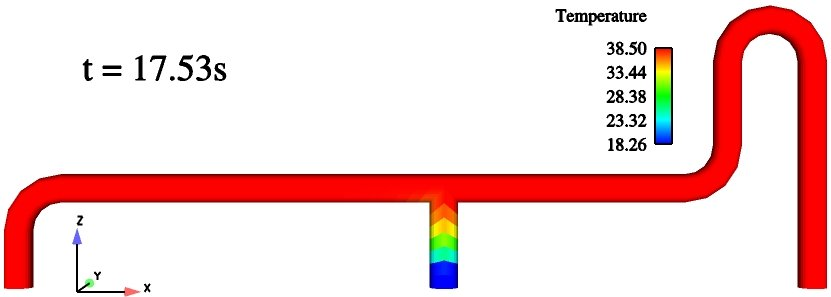
\includegraphics[width=10cm]{case5_05} \\
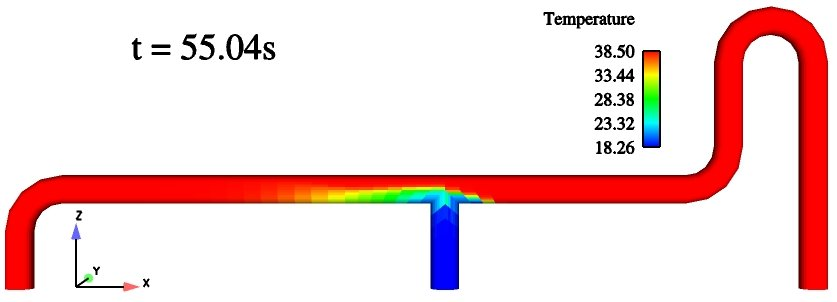
\includegraphics[width=10cm]{case5_06} \\
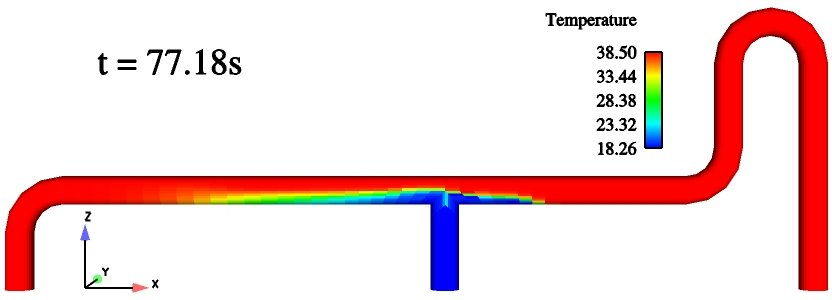
\includegraphics[width=10cm]{case5_07} \\
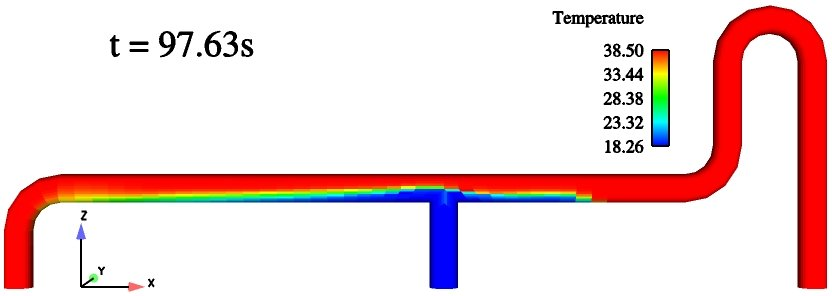
\includegraphics[width=10cm]{case5_08} \\
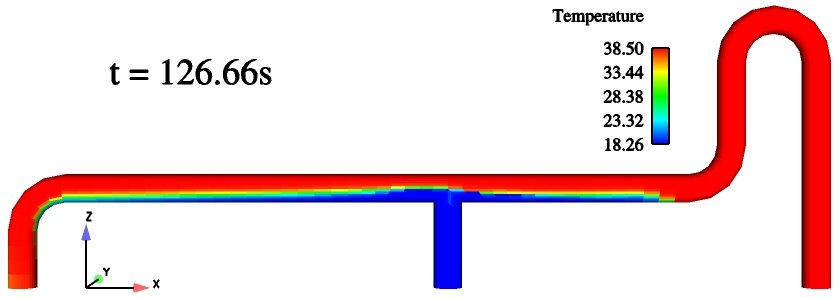
\includegraphics[width=10cm]{case5_09} \\
\end{tabular}
\caption{Evolution of temperature}
\label{fige2_e5}
\end{center}
\end{figure}



Figure \ref{fige4_e5} shows the cells where the temperature
is lower than 21\degresC. It is not an isosurface created from the full domain,
but a visualization of the full sub-domain created through the post-processing
routines.

\begin{figure}[h!]
\begin{center}
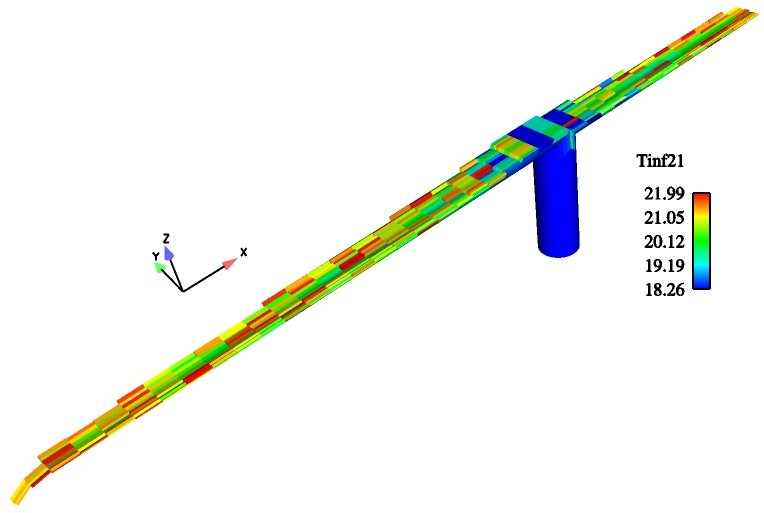
\includegraphics[width=10cm]{case5_03}
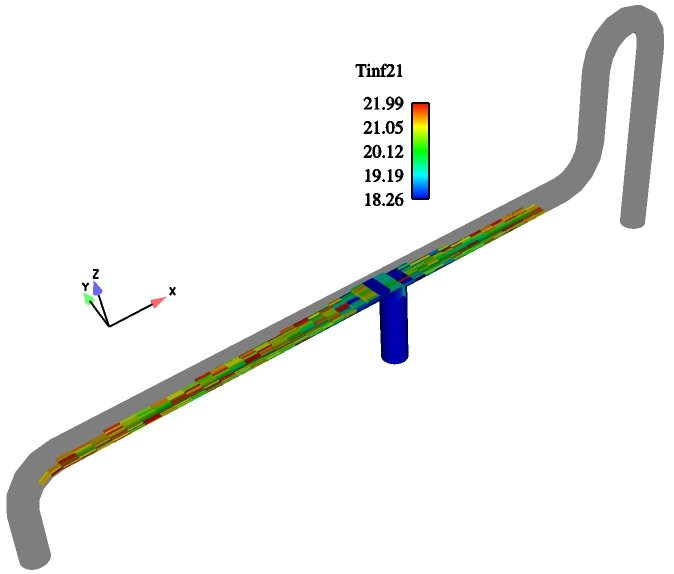
\includegraphics[width=10cm]{case5_04}
\caption{Sub-domain where the temperature is lower than 21\degresC\ (upper figure)
and localization in the full domain (lower figure)}
\label{fige4_e5}
\end{center}
\end{figure}

\setcounter{section}{0}
\stepcounter{chapter}
\part{STEP BY STEP SOLUTION}
%-------------------------------------------------------------------------------

% This file is part of Code_Saturne, a general-purpose CFD tool.
%
% Copyright (C) 1998-2013 EDF S.A.
%
% This program is free software; you can redistribute it and/or modify it under
% the terms of the GNU General Public License as published by the Free Software
% Foundation; either version 2 of the License, or (at your option) any later
% version.
%
% This program is distributed in the hope that it will be useful, but WITHOUT
% ANY WARRANTY; without even the implied warranty of MERCHANTABILITY or FITNESS
% FOR A PARTICULAR PURPOSE.  See the GNU General Public License for more
% details.
%
% You should have received a copy of the GNU General Public License along with
% this program; if not, write to the Free Software Foundation, Inc., 51 Franklin
% Street, Fifth Floor, Boston, MA 02110-1301, USA.

%-------------------------------------------------------------------------------

\section{SOLUTION FOR CASE 1}
The first thing to do before running \CS is to prepare the computation
directories. In this first example, the study directory ``T\_JUNCTION'' will be
created, containing a single calculation directory CAS1. This is done by typing
the command:
\begin{center}
\texttt{code\_saturne create -s T\_JUNCTION -c CASE1}\
\end{center}
The mesh files should be copied in the directory MESH.

The \CS Graphical Interface is launched by typing the command
{\itshape ./SaturneGUI} in the DATA subdirectory of the CAS1 directory.
The following graphic window opens (fig \ref{fig1_e1}).

\begin{figure}[ht]
\begin{center}
\includegraphics[width=13cm]{V-1}
\caption{User interface}
\label{fig1_e1}
\end{center}
\end{figure}


\clearpage
Go to the {\itshape File} menu and click on {\itshape New file} to open a new
calculation data file, as shown in the figure
\ref{fig2_e1}.

\begin{figure}[ht]
\begin{center}
\includegraphics[width=13cm]{V-2}
\caption{Opening a new file}
\label{fig2_e1}
\end{center}
\end{figure}


\clearpage
The interface automatically updates the following information:
\begin{itemize}
        \item Study name
        \item Case name
        \item Directory of the case
        \item Associated sub-directories of the case
\end{itemize}

\begin{figure}[ht]
\begin{center}
\includegraphics[width=12cm]{V-3}
\caption{Identity and paths}
\label{fig3_e1}
\end{center}
\end{figure}


\clearpage
Save the case to give a name to the new {\itshape XML file} by opening the
{\itshape File} menu and clicking on {\itshape Save as...}. A new window will
appear, enter the name of the case in {\itshape File Name} then click on
{\itshape Save}.

Remember to save the case regularly throughout the preparation of the calculation.

\begin{figure}[ht]
\begin{center}
\includegraphics[width=10cm]{V-4}
\caption{Saving the {\itshape XML} file}
\label{fig4_e1}
\end{center}
\end{figure}


\clearpage
The next step is to specify the mesh(es) to be used for the calculation.
Click on the item {\itshape Solution Domain}
under the heading {\itshape Analysis environment}. The list of all
meshes available in the folder {\itshape MESH} appears in the
window {\itshape List of meshes}. Delete the mesh(es) you will not
use\footnote{this operation only deletes the selected entries from the list, it
does not delete the mesh file in the MESH directory}. In this case only the
mesh {\itshape downcomer.des} is needed.

\begin{figure}[ht]
\begin{center}
\includegraphics[width=12cm]{V-5}
\caption{Meshes: list of meshes}
\label{fig5_e1}
\end{center}
\end{figure}

On this item ({\itshape Solution Domain}) there are three other tabs:
\begin{itemize}
        \item PERIODIC BOUNDARIES
        \item SYRTHES COUPLING
        \item STAND-ALONES RUNNING
\end{itemize}
They are not used in this case. Keep the default values.

\clearpage
The item {\itshape Analysis features} under the heading {\itshape Thermophysical
environment} allows to define the type of flow to be simulated. In this case, a
steady flow will be chosen.

\begin{figure}[ht]
\begin{center}
\includegraphics[width=12cm]{V-6}
\caption{Flow type}
\label{fig7_e1}
\end{center}
\end{figure}


\clearpage
The turbulence model is selected in the following list:\\
\hspace*{1cm}$\bullet\ $laminar flow (no model)\\
\hspace*{1cm}$\bullet\ $mixing length\\
\hspace*{1cm}$\bullet\ $k-$\varepsilon$\\
\hspace*{1cm}$\bullet\ $k-$\varepsilon$ Linear Production\\
\hspace*{1cm}$\bullet\ $Rij-$\varepsilon$ LLR\\
\hspace*{1cm}$\bullet\ $Rij-$\varepsilon$ SSG\\
\hspace*{1cm}$\bullet\ $v2f ($\varphi$ model)\\
\hspace*{1cm}$\bullet\ $k-$\omega$ SST\\
\hspace*{1cm}$\bullet\ $LES (Smagorinsky)\\
\hspace*{1cm}$\bullet\ $LES (dynamic model)

\begin{figure}[ht]
\begin{center}
\includegraphics[width=12cm]{V-7}
\caption{Turbulence model: list of models}
\label{fig9_e1}
\end{center}
\end{figure}


\clearpage
In this case, the k-$\varepsilon$ model is used.

\begin{figure}[ht]
\begin{center}
\includegraphics[width=9cm]{V-8}
\caption{Turbulence model: choice of a model}
\label{fig10_e1}
\end{center}
\end{figure}


\clearpage
For this study the equation for temperature must be solved. Click on the item
{\itshape Thermal model} to
choose between:\\
\hspace*{1cm}$\bullet\ $No thermal scalar\\
\hspace*{1cm}$\bullet\ $Temperature (Celsius degrees)\\
\hspace*{1cm}$\bullet\ $Temperature (Kelvin)\\
\hspace*{1cm}$\bullet\ $Enthalpy

\begin{figure}[ht]
\begin{center}
\includegraphics[width=12cm]{V-9}
\caption{Thermal scalar conservation: list of models}
\label{fig11_e1}
\end{center}
\end{figure}


\clearpage
In the present case, select {\itshape Temperature (Celsius degrees)}.
\begin{figure}[ht]
\begin{center}
\includegraphics[width=9cm]{V-10}
\caption{Thermal scalar conservation: choice of a model}
\label{fig12_e1}
\end{center}
\end{figure}

Once the thermal scalar selected, additional items appear.
There are no radiative transfers in our case, so this item can be ignored.

\clearpage
To initialize the thermal scalar, go to the item
{\itshape Definition and Initialization} under the heading
{\itshape Additional scalars}, where more options concerning the scalars can be
specified. The value of the initial value can be modified in any of the two
pages. But in case there are additional scalars ({\em i.e.} other than the
thermal scalar), their initialization is only possible in the {\itshape
Additional scalars} page.

\begin{figure}[ht]
\begin{center}
\includegraphics[width=12cm]{V-12}
\caption{Initialization of the scalar}
\label{fig15_e1}
\end{center}
\end{figure}


\clearpage
Click on the thermal scalar in the list, to change:
\begin{itemize}
        \item its name
        \item its initial value
        \item its minimal value
        \item its maximal value
\end{itemize}
In this case the temperature can vary between 0\degresC\ and 400\degresC.

\begin{figure}[ht]
\begin{center}
\includegraphics[width=8cm]{V-13}
\caption{Initialization of the scalar}
\label{fig16_e1}
\end{center}
\end{figure}

The item {\itshape Physicals properties} under the heading {\itshape Additional
scalars}\footnote{not to be confused with the heading {\itshape Physical
properties} in the main list} is used to specify the physical properties
of the additional scalars, {\em i.e.} those that are not the thermal scalar. In
this case there are no additional scalars, the item is therefore unused.


\clearpage
Under the heading {\itshape Physical properties} in the main list,
the item {\itshape Reference values} allows to set the reference pressure.
Use the default value of $101\,300\ Pa$.

\begin{figure}[ht]
\begin{center}
\includegraphics[width=12cm]{V-14}
\caption{Physical properties: reference pressure}
\label{fig17_e1}
\end{center}
\end{figure}


\clearpage
Specify the fluid physical characteristics in the item {\itshape Fluid
properties}:
\begin{itemize}
        \item Density
        \item Viscosity
        \item Specific Heat
        \item Thermal Conductivity
\end{itemize}

In this case they are all constant.
\begin{itemize}
        \item Density $ = 725.735\ kg.m^{-3}$
        \item Viscosity $ = 0.895\times 10^{-4}\ kg.m^{-1}.s^{-1}$
        \item Specific Heat $  = 5\,483\ J.kg^{-1}.\mbox{\degresC}^{-1}$
        \item Thermal Conductivity $ = 0.02495\ W.m^{-1}.K^{-1}$
\end{itemize}

\begin{figure}[ht]
\begin{center}
\includegraphics[width=12cm]{V-15}
\caption{Physical properties: fluid properties}
\label{fig18_e1}
\end{center}
\end{figure}


\clearpage
Set the three components of gravity in the
{\itshape Gravity, hydrostatic pressure} item.
In this case, since the gravity doesn't have
any influence on the flow, gravity can be set to 0.
As for the pressure interpolation method, keep the standard
default value.

\begin{figure}[ht]
\begin{center}
\includegraphics[width=12cm]{V-16}
\caption{Physical properties: gravity, hydrostatic pressure}
\label{fig19_e1}
\end{center}
\end{figure}

\clearpage
To initialize variables at the instant $t=0\ s$, go to the item {\itshape Initialization} under the heading {\itshape Volume conditions}.
Here the velocity, the thermal scalar and the turbulence can be initialized. In
this case, the default values can be kept: zero velocity, an initial temperature
of 20\degresC\ (consistant with previous initialization) and a turbulence level based on a reference velocity of $1\
m.s^{-1}$. Specific zones can be defined with different initializations. In this
case, only the default ``all cells'' is used.

\begin{figure}[ht]
\begin{center}
\includegraphics[width=12cm]{V-11}
\caption{Initialization of dynamic variables}
\label{fig14_e1}
\end{center}
\end{figure}



\clearpage
Boundary conditions now need to be defined. Go to the item {\itshape Define
boundary regions} under the heading {\itshape Boundary conditions}.
The following window opens (fig \ref{fig20_e1}).

\begin{figure}[ht]
\begin{center}
\includegraphics[width=12cm]{V-17}
\caption{Creation of a boundary region}
\label{fig20_e1}
\end{center}
\end{figure}


\clearpage
Each boundary must be defined. Click on {\itshape Add} to edit a new boundary. 
The boundary faces will be grouped in
user-defined zones, based on their color or on geometrical conditions. For each
zone, a reference number, a label, a nature and a selection criteria must be
assigned.
The different natures that can be assigned are:\\
\hspace*{1cm}$\bullet\ $wall\\
\hspace*{1cm}$\bullet\ $inlet\\
\hspace*{1cm}$\bullet\ $symmetry\\
\hspace*{1cm}$\bullet\ $outlet

The {\itshape Label} can be any character string. It is used to identify the
zone more easily. It usually corresponds to the nature of the zone.

The {\itshape Zone} number can be any integer. It will be used by the code to
identify the zone. No specific order or continuity in the numbering is needed.

The {\itshape Selection criteria} is used to define the faces that belong to the
zone. It can be a color number, a group reference, geometrical conditions, on a
combination of them, related by ``or'' or ``and'' keywords.

\begin{figure}[ht]
\begin{center}
\includegraphics[width=8cm]{V-18}
\caption{Creation of a boundary region}
\label{fig21_e1}
\end{center}
\end{figure}


\clearpage
The specification of the inlet condition is detailled in the following
pages. The settings will be as follows:\\
\hspace*{1cm}$\bullet\ ${\itshape Label}: inlet\\
\hspace*{1cm}$\bullet\ ${\itshape Zone}: 1\\
\hspace*{1cm}$\bullet\ ${\itshape Nature}: inlet\\
\hspace*{1cm}$\bullet\ ${\itshape Selection criteria}: 1

Type all the information in the fields, the result diplays as figure \ref{fig20_e1}

\begin{figure}[ht]
\begin{center}
\includegraphics[width=8cm]{V-20}
\caption{Creation of a boundary region}
\label{fig20_e1}
\end{center}
\end{figure}

Remember to save the Xml file regularly!


\clearpage
Do the same thing for the other boundaries.

In our case, colors 8 and 9 are symmetry boundaries. One option can be to define
a separate zone for each color, as follows:
\begin{center}
\begin{tabular}{lcp{2cm}c}
Label & symmetry\_1 & & symmetry\_2 \\
Zone & 3 & & 4 \\
Nature & symmetry & & symmetry \\
Localization & 8 & & 9 \\
\end{tabular}
\end{center}

But it is usually faster to regroup the different colors in one single zone, as
shown on figure \ref{fig24_e1}. In our case, the localization for this zone is
the string ``8 or 9''.

\begin{figure}[ht]
\begin{center}
\includegraphics[width=8cm]{V-21}
\caption{Creation of boundary regions: symmetry region}
\label{fig24_e1}
\end{center}
\end{figure}


\clearpage
The same treatment must be done for the wall conditions. All colors 2, 3, 4, 6
and 7 can be grouped in a single boundary zone.

After defining all the boundary zones, the Interface window will look as in
figure \ref{fig25_e1}.

\begin{figure}[ht]
\begin{center}
\includegraphics[width=8cm]{V-22}
\caption{Creation of boundary regions}
\label{fig25_e1}
\end{center}
\end{figure}


\clearpage
Now that the boundary zones are defined, the boundary conditions assigned to
them will be specified. Click on the item
{\itshape Boundary conditions} to set the inlet boundary conditions for
velocity and turbulence. As shown on figure \ref{fig26_e1}, outlet and wall boundary zones also appear in the window.

\begin{figure}[ht]
\begin{center}
\includegraphics[width=12cm]{V-23}
\caption{Dynamic variables boundary conditions}
\label{fig26_e1}
\end{center}
\end{figure}


\clearpage
Click on the label {\itshape inlet}. In the section {\itshape Velocity}, select {\itshape norm}, then in the sub-section {\itshape Direction} choose {\itshape specified ccordinates} and enter the normal vector components of the inlet
velocity. For the turbulence, chose the inlet condition based on a hydraulic
diameter and specify it.\\
\hspace*{1cm}$\bullet\ X = 1\ m$\\
\hspace*{1cm}$\bullet\ Y = 0\ m$\\
\hspace*{1cm}$\bullet\ Z = 0\ m$\\
\hspace*{1cm}$\bullet\ D = 0.5\ m$

\begin{figure}[ht]
\begin{center}
\includegraphics[width=9cm]{V-24}
\caption{Dynamic variables boundary: inlet}
\label{fig27_e1}
\end{center}
\end{figure}


\clearpage
As for the wall boundary zone, the specifications the user might have to
give is when the wall is sliding, and if the wall is "smooth" or "rough". In this case, the walls are fixed so the
option is not selected, and the wall is considered as "smooth".

Note that if one of the walls had been sliding, it would have been necessary to
isolate the corresponding boundary faces in a specific boundary region.

\begin{figure}[ht]
\begin{center}
\includegraphics[width=9cm]{V-25}
\caption{Dynamic variables boundary: walls}
\label{fig28_e1}
\end{center}
\end{figure}


\clearpage
The boundary conditions
on the temperature are only applied on inlets, outlets and walls.

For the walls, three conditions are available:\\
\hspace*{1cm}$\bullet\ ${\itshape Prescribed value}\\
\hspace*{1cm}$\bullet\ ${\itshape Prescribed flux}\\
\hspace*{1cm}$\bullet\ ${\itshape Exchange Coefficient}

For the outlet, only {\itshape Prescribed value} and {\itshape Prescribed flux} are available, but they are
taken into account only when the flow re-enters from the outlet. Otherwise,
homogeneous {\itshape Prescribed flux} is considered by \CS.

For the inlets, only {\itshape Prescribed value} is available.

In this case all walls are adiabatic. So the boundary condition for the
temperature will be a {\itshape Prescribed flux} set to 0.
\begin{figure}[ht]
\begin{center}
\includegraphics[width=10cm]{V-27}
\caption{Scalars boundaries: walls}
\label{fig30_e1}
\end{center}
\end{figure}


\clearpage
Click on {\itshape inlet} to choose the temperature inlet
value. Here this value is 300\degresC.
The default value is left for the outlet.

\begin{figure}[ht]
\begin{center}
\includegraphics[width=10cm]{V-28}
\caption{Scalars boundaries: inlet}
\label{fig31_e1}
\end{center}
\end{figure}


\clearpage
The calculation parameters need then to be specified, under the header {\itshape
Numerical parameters}.

Go to the item {\itshape Steady flow management} to specify the number of iterations,
30 in this case. The default value of the relaxation
coefficient will be kept and  the {\itshape Zero iteration option} 
will not be activated.

\begin{figure}[ht]
\begin{center}
\includegraphics[width=12cm]{V-29}
\caption{Steady flow management}
\label{fig32_e1}
\end{center}
\end{figure}


\clearpage
After selecting the item {\itshape Equation parameters}, the tab {\itshape Scheme} allows to change different more
advanced numerical parameters. In this case none of them should be changed from
their default value.

\begin{figure}[!h]
\begin{center}
\includegraphics[width=11cm]{V-34}
\caption{Numerical parameters}
\label{fig3738_e1}
\end{center}
\end{figure}

\begin{figure}[!h]
\begin{center}
\includegraphics[width=11cm]{V-34bis}
\caption{Numerical parameters}
\label{fig3738bis_e1}
\end{center}
\end{figure}

\clearpage
Under the heading {\itshape Calculation control}, click on the item {\itshape Output control} to change the frequency for the
printing of information in the output listing.
The options are:\\
\hspace*{1cm}$\bullet\ ${\itshape No output}\\
\hspace*{1cm}$\bullet\ ${\itshape Output listing at each time step}\\
\hspace*{1cm}$\bullet\ ${\itshape Output at each 'n' time step} (the value of
'n' must then be specified)\\
Here and in most cases, the second option should be chosen.

\begin{figure}[ht]
\begin{center}
\includegraphics[width=12cm]{V-30}
\caption{Output control: output listing}
\label{fig33_e1}
\end{center}
\end{figure}


\clearpage
For the post-processing (by default EnSight format files), there are three options:\\
\hspace*{1cm}$\bullet\ ${\itshape Only at the end of calculation}\\
\hspace*{1cm}$\bullet\ ${\itshape At each time step}\\
\hspace*{1cm}$\bullet\ ${\itshape Post-processing every 'n' time steps}

In this case, we are interested in the evolution of the variables during the
calculation, so the second option is chosen.

\begin{figure}[ht]
\begin{center}
\includegraphics[width=8cm]{V-31}
\caption{Output control: post-processing}
\label{fig34_e1}
\end{center}
\end{figure}


\clearpage
The other options are kept to their default value.

\begin{figure}[ht]
\begin{center}
\includegraphics[width=8cm]{V-32}
\caption{Output control}
\label{fig35_e1}
\end{center}
\end{figure}

The {\itshape Monitoring Points Coordinates} tab allows to define specific points
in the domain (monitoring probes) where the time evolution of the different
variables will be stored in historic files. In this case no monitoring points
are defined.


\clearpage
The item {\itshape Volume solution control} allows to specify which variable will
appear in the output listing, in the post-processing files or on the
monitoring probes. In this case, the default value is kept, where every variable
is activated.


\begin{figure}[ht]
\begin{center}
\includegraphics[width=12cm]{V-33}
\caption{Solution control}
\label{fig36_e1}
\end{center}
\end{figure}


\clearpage
When using Fortran routines, it is sometimes useful to allocate pre-defined user
arrays, that are present in every sub-routine. This allocation can be specified
in the {\itshape User arrays} item, under the {\itshape Calculation management}
heading. It is not the case in the present calculation.\\

The item {\itshape Memory management} allows to set the
memory size for the calculation. It is the size of the integer and real arrays that will be used to store most of the variables in the Fortran parts of \CS.
It is dependent on the number of cells in the mesh. In parallel mode, it depends
on the number of cells treated by each processor, and not the total number of
cells. For this simple case, the default values are appropriate.

\begin{figure}[ht]
\begin{center}
\includegraphics[width=12cm]{V-35}
\caption{User arrays}
\label{fig39_e1}
\end{center}
\end{figure}


\clearpage
The item {\itshape Start/Restart} allows to start a new calculation from the
results of a former one. It is not the case in the present calculation so
nothing has to be modified.

\begin{figure}[ht]
\begin{center}
\includegraphics[width=12cm]{V-36}
\caption{Start/Restart}
\label{fig40_e1}
\end{center}
\end{figure}


\clearpage
The final item, {\itshape Prepare batch calculation}, is used to prepare the launch
script and, on certain architectures, launch the calculation.

Calculations can be launched from the Graphical Interface in interactive mode
({\itshape Workstation}) or in a PBS batch queue ({\itshape Management of chart
PBS}). In this simple case, choose the Workstation.

\begin{figure}[ht]
\begin{center}
\includegraphics[width=10cm]{V-37}
\caption{Prepare batch analysis: Computer selection}
\label{fig41_e1}
\end{center}
\end{figure}


\clearpage
Click on the icon to {\itshape Select the batch script file} to select the
launch script. The default launch script is named {\itshape runcase} and is
located in the SCRIPTS directory. Select it and click on {\itshape Open}.

Remember to save the Xml file before opening the launch script.

\begin{figure}[ht]
\begin{center}
\includegraphics[width=12cm]{V-38}
\caption{Prepare batch analysis: Batch script file selection}
\label{fig42_e1}
\end{center}
\end{figure}


\clearpage
When the script is selected, new options will appear.
On this calculation, the number of processors used will be left to 1.

When launching a calculation, a temporary directory is created on the machine,
where the script copies and creates temporary files and from where the \CS
executable is launched. Should some user routines read or write case-specific
files, they must be copied in the temporary directory, or from the temporary
directory into the RESU directory. The {\itshape User files} icon allows the
user to specify user data files (in the DATA directory) or user result files,
that will then be copied automatically to or from the temporary directory.
In this example, no user file is needed.

Finally, the {\itshape Advanced options} icon allows to change some more
advanced parameters that will not be needed in this simple case.

Eventually, save the Xml file and execute it by clicking on
\CS {\itshape batch running}. The results will be copied in the RESU
directory.

\begin{figure}[ht]
\begin{center}
\includegraphics[width=10cm]{V-39}
\caption{Prepare batch analysis: Execution}
\label{fig43_e1}
\end{center}
\end{figure}



%-------------------------------------------------------------------------------

% This file is part of Code_Saturne, a general-purpose CFD tool.
%
% Copyright (C) 1998-2012 EDF S.A.
%
% This program is free software; you can redistribute it and/or modify it under
% the terms of the GNU General Public License as published by the Free Software
% Foundation; either version 2 of the License, or (at your option) any later
% version.
%
% This program is distributed in the hope that it will be useful, but WITHOUT
% ANY WARRANTY; without even the implied warranty of MERCHANTABILITY or FITNESS
% FOR A PARTICULAR PURPOSE.  See the GNU General Public License for more
% details.
%
% You should have received a copy of the GNU General Public License along with
% this program; if not, write to the Free Software Foundation, Inc., 51 Franklin
% Street, Fifth Floor, Boston, MA 02110-1301, USA.

%-------------------------------------------------------------------------------

\section{SOLUTION FOR CASE 2}
This case corresponds to a new study, in which there will be three calculation
cases (cases 2, 3 and 4). All of them can be created in a single {\itshape
code\_saturne create} command, or additional cases can be added later. To test both
possibilities, first create the study directory, with cases directories CAS2
and CAS4:\\
{\itshape code\_saturne create -s FULL\_DOMAIN CAS2 CAS4}\\
then go in the study directory and add the CAS3 directory:\\
{\itshape cd FULL\_DOMAIN}\\
{\itshape code\_saturne create -c CAS3}

Go to the DATA directory in CAS2,
open a new case and select the meshes to use. Click on the
heading {\itshape Calculation environment} then on the item {\itshape Meshes selection}. In this case the three meshes have to be
joined. So don't delete any mesh and activate the {\itshape Join meshes} option by clicking in the box. Additional information appears on the page. If it is
left untouched, the \CS Preprocessor will test all the boundary faces for
potential joining (based on geometrical criteria). To make mesh joining more
efficient, this analysis can be restricted to a sub-set of boundary faces. This
is the case in the present calculation, since only faces of colors 5, 24 and 32
are liable to be joined.

Click on the {\itshape New} icon to enter the list of colors to be joined.

\begin{figure}[h!]
\begin{center}
\includegraphics[width=12cm]{V-40}
\caption{Meshes: list of meshes}
\label{fig2_e2}
\end{center}
\end{figure}


\newpage
Fill the array
{\itshape References} for the color reference to be joined: 5, 24 and 32.
(different colors can be entered on a single line, separated by blanks).

\begin{figure}[h!]
\begin{center}
\includegraphics[width=12cm]{V-41}
\caption{Join a Mesh}
\label{fig5_e2}
\end{center}
\end{figure}


\newpage
In this case ``Unsteady flow'' must be selected in the
{\itshape Analysis features} item.

\begin{figure}[h!]
\begin{center}
\includegraphics[width=12cm]{V-43}
\caption{Thermophysical models - Analysis features - Unsteady flow}
\label{fig6_e2}
\end{center}
\end{figure}

The rest of the heading {\itshape Thermophysical models} is identical to case
1.


\newpage
To add an additional scalar, click on the
{\itshape Definition and Initialization} item under the
{\itshape Additional scalars} heading.
The characteristics of the thermal scalar are still the
same. Its initial value is 20\degresC\ and it can vary between
0\degresC\ and 400\degresC.

To create an additional scalar, click on {\itshape Add}, then enter:\\
\hspace*{1cm}$\bullet\ $its {\itshape Name}: scalar\_2\\
\hspace*{1cm}$\bullet\ $its {\itshape Initial value}: 10\\
\hspace*{1cm}$\bullet\ $its {\itshape Minimal value}: 0\\
\hspace*{1cm}$\bullet\ $its {\itshape Maximal value}: 400


\begin{figure}[h!]
\begin{center}
\includegraphics[width=12cm]{V-44}
\caption{Additional scalar - User scalar definition}
\label{fig8_e2}
\end{center}
\end{figure}


\newpage
In the item {\itshape Physical properties}, still under the heading
{\itshape Additional scalars}, specify the diffusion coefficient of this new
scalar. Click on the scalar name to highlight it, then enter the value in the
box. In this case, the value is
$0.895\times 10^{-4}\ m^{2}.s^{-1}$

\begin{figure}[h!]
\begin{center}
\includegraphics[width=12cm]{V-45}
\caption{Additional scalar - User scalar physical properties}
\label{fig9_e2}
\end{center}
\end{figure}


\newpage
Create the boundary zones. The procedure is the same as in case 1, but the
colors are different. Note that colors 5 and 32 have completely disappeared in
the joining process (they are now internal faces and are not considered as
boundaries), while some boundary faces of color 24 remain.\\
Create the inlet, outlet
and symmetry boundary zones with the following colors:\\
\hspace*{1cm}$\bullet\ $inlet: color 1\\
\hspace*{1cm}$\bullet\ $outlet: color 34\\
\hspace*{1cm}$\bullet\ $symmetry: colors 8 9 28 29 38 39\\

\begin{figure}[h!]
\begin{center}
\includegraphics[width=12cm]{V-46}
\caption{Creation of the boundary zones}
\label{fig10_e2}
\end{center}
\end{figure}


\newpage
In this case, different conditions are applied for the walls. Separate
corresponding wall boundary regions must therefore be created, following the
data in the following table.

\begin{center}
\begin{tabular}{cccc}
Label & Zone & Nature & Localization \\
wall\_2 & 5 & wall & 2 or 3 \\
wall\_3 & 6 & wall & 4 or 7 or 21 or 22 or 23 \\
wall\_4 & 7 & wall & 6 and Y$>$1 \\
wall\_5 & 8 & wall & 6 and Y$\leqslant$1 \\
wall\_6 & 9 & wall & 31 or 33 \\
\end{tabular}
\end{center}

The ``wall\_1'' region combines color and geometrical criteria. The associated
character string to enter in the ``Selection criteria'' box is as follows:\\
``24 and 0.1$<$=X and 0.5$>$=X''\footnote{Note that, due to the joining process,
there are in fact no boundary faces of color 24 with X coordinate outside the
[0.1;0.5] intervalle. The geometrical criterium is therefore not
necessary. It is presented here to show the capacity of the face selection
module}.

\begin{figure}[h!]
\begin{center}
\includegraphics[width=10cm]{V-47}
\caption{Creation of a wall boundary region}
\label{fig11_e2}
\end{center}
\end{figure}


\newpage
Define the other wall boundary zones. The faces of color 6 have to be divided in
two separate zones, based on a geometrical criterium on $Y$.

\begin{figure}[h!]
\begin{center}
\includegraphics[width=9cm]{V-48}
\caption{Creation of wall boundary regions}
\label{fig152_e2}
\end{center}
\end{figure}


\newpage
The dynamic boundary conditions are the same as in case 1 for the inlet, and
there are still no sliding walls.


\begin{figure}[h!]
\begin{center}
\includegraphics[width=12cm]{V-49}
\caption{Dynamic variables boundary: inlet}
\label{fig16_e2}
\end{center}
\end{figure}


\newpage
To configure the scalar boundary conditions on the walls, select individually each wall in the item {\itshape Boundary conditions}.
On all the walls, a default homogeneous prescribed flux is set for
temperature, and prescribed values are specified for the passive scalar,
according to the following table:
\begin{center}
\begin{tabular}{|c|c|c|}
\hline
Wall & Nature & Value \\
\hline
wall\_1 & Prescribed value  & 0 \\
\hline
wall\_2 & Prescribed value  & 5 \\
\hline
wall\_3 & Prescribed value  & 0 \\
\hline
wall\_4 & Prescribed value  & 25 \\
\hline
wall\_5 & Prescribed value  & 320 \\
\hline
wall\_6 & Prescribed value  & 40 \\
\hline
\end{tabular}
\end{center}

\begin{figure}[h!]
\begin{center}
\includegraphics[width=9cm]{V-50}
\caption{Scalars boundaries: wall\_5}
\label{fig21_e2}
\end{center}
\end{figure}


\newpage
Click on {\itshape inlet}, to set the inlet values for the scalars: 300\degresC\
for temperature and 200 for the passive scalar.

\begin{figure}[h!]
\begin{center}
\includegraphics[width=8cm]{V-51}
\caption{Scalars boundaries: inlet}
\label{fig22_e2}
\end{center}
\end{figure}


\newpage
Some calculation parameters now need to be defined.
Go to the item {\itshape Time step} under the heading
{\itshape Numerical parameters}. In our case the time step is
{\itshape Uniform and constant}. Set the number of iterations to 300 and the
reference time step to $0.05\ s$.

\begin{figure}[h!]
\begin{center}
\includegraphics[width=12cm]{V-52}
\caption{Time step setting}
\label{fig23_e2}
\end{center}
\end{figure}

No change is needed in the {\itshape Equation parameters} and {\itshape Global parameters} items.

\newpage
Go to the item {\itshape Output control} under the heading {\itshape Calculation control} to set the output parameters.

Keep the default value for the output listing frequency.

For the Post-processing, select the third option (output every 'n' time steps)
and set the value of 'n' to 2.

Activate the post-processing on the boundary faces by ticking the
{\itshape Domain boundary post processing} box. The EnSight format file will
contain an additional part, composed of the boundary faces, on which boundary
conditions and some other variables can be visualized. This allows to check if
the boundary conditions for the passive scalar have been properly set.

\begin{figure}[h!]
\begin{center}
\includegraphics[width=12cm]{V-53}
\caption{Output control: post-processing}
\label{fig24_e2}
\end{center}
\end{figure}


\newpage
In this case, chronological records on specified monitoring probes are needed.
To define the probes, click on the
{\itshape Monitoring points Coordinates} tab.

\begin{figure}[h!]
\begin{center}
\includegraphics[width=12cm]{V-54}
\caption{Output control: monitoring points}
\label{fig25_e2}
\end{center}
\end{figure}



\newpage
Click on ``Add'' and enter the coordinates of the monitoring points you want to define. For the first point:\\
\hspace*{1cm}$\bullet\ X = -0.25\ m$\\
\hspace*{1cm}$\bullet\ Y = 2.25\ m$\\
\hspace*{1cm}$\bullet\ Z = 0\ m$


\begin{figure}[h!]
\begin{center}
\includegraphics[width=8cm]{V-56}
\caption{Output controls: monitoring points - $1^{st}$ point}
\label{fig27_e2}
\end{center}
\end{figure}


\newpage
Repeat the procedure for the other probes. Their coordinates are indicated in
the following table (the Z coordinate is always 0).
\begin{center}
\begin{tabular}{|c|c|c|}
\hline
Points & X(m) & Y(m) \\
\hline
2 & 0.05 & 2.25 \\
\hline
3 & 0.05 & 2.75 \\
\hline
4 & 0.05 & 0.5 \\
\hline
5 & 0.05 & -0.25 \\
\hline
6 & 0.75 & -0.25 \\
\hline
7 & 0.75 & 0.25 \\
\hline
8 & 0.75 & 0.75 \\
\hline
\end{tabular}
\end{center}

\begin{figure}[h!]
\begin{center}
\includegraphics[width=9cm]{V-57}
\caption{Output control: monitoring points}
\label{fig28_e2}
\end{center}
\end{figure}

Remember to save the Xml file regularly.


\newpage
Go to the item {\itshape Volume solution control} to define which variables will
appear in the listing, the post-processing and the chronological records.

Uncheck the boxes in front of the {\itshape Pressure}, {\itshape Tubulent energy}
and {\itshape Dissipation} variables, in the {\itshape  Print in listing}
column. Information on these three variables will not appear in the output
listing anymore.

Uncheck the boxes in front of the {\itshape Courant number} and {\itshape
Fourier number} variables in the {\itshape Post-processing} column. These
variables will be removed from the post-processing results.

\begin{figure}[h!]
\begin{center}
\includegraphics[width=12cm]{V-58}
\caption{Solution control - Output configuration}
\label{fig29_e2}
\end{center}
\end{figure}


\newpage
Delete all the probe numbers for the {\itshape total\_pressure} variable. No
chronological record will be created for this variable. As for the
{\itshape VelocitX} variable, only select probes  1, 2, 6, 7 and 8. Time
evolution on the other probes will not be recorded.

\begin{figure}[h!]
\begin{center}
\includegraphics[width=10cm]{V-59}
\caption{Solution control - Probes}
\label{fig30_e2}
\end{center}
\end{figure}


Switch to the {\itshape Calculation management} heading to prepare the launch
script and run the calculation.


%                      Code_Saturne version 1.3
%                      ------------------------
%
%     This file is part of the Code_Saturne Kernel, element of the
%     Code_Saturne CFD tool.
%
%     Copyright (C) 1998-2008 EDF S.A., France
%
%     contact: saturne-support@edf.fr
%
%     The Code_Saturne Kernel is free software; you can redistribute it
%     and/or modify it under the terms of the GNU General Public License
%     as published by the Free Software Foundation; either version 2 of
%     the License, or (at your option) any later version.
%
%     The Code_Saturne Kernel is distributed in the hope that it will be
%     useful, but WITHOUT ANY WARRANTY; without even the implied warranty
%     of MERCHANTABILITY or FITNESS FOR A PARTICULAR PURPOSE.  See the
%     GNU General Public License for more details.
%
%     You should have received a copy of the GNU General Public License
%     along with the Code_Saturne Kernel; if not, write to the
%     Free Software Foundation, Inc.,
%     51 Franklin St, Fifth Floor,
%     Boston, MA  02110-1301  USA
%
%-----------------------------------------------------------------------
\section{SOLUTION FOR CASE 3}

Only a few elements are different from case 2.

In this case the density becomes variable. Go to the item
{\itshape Fluid properties} under the heading
{\itshape Physical properties} and change the nature of the density from
{\itshape constant} to {\itshape variable}.

\begin{figure}[h!]
\begin{center}
\includegraphics[width=12cm]{\repgraphics/c3_capture01.jpg}
\caption{Fluid properties - Variable density}
\label{fig1_e3}
\end{center}
\end{figure}


\newpage
As the density is variable, the influence of gravity has to be considered. In the
heading {\itshape Physical properties} go to
{\itshape Gravity, hydrostatic pressure} and set the value of each component of
the gravity vector. If the norm of gravity is the standard $9.81\ m.s^{-2}$, a
alternative way to define gravity is to specify its direction in the component
boxes, (0;-1;0) in our case, and click on the icon below to renormalize the
vector to 9.81.

\begin{figure}[h!]
\begin{center}
\includegraphics[width=12cm]{\repgraphics/c3_capture02.jpg}
\caption{Fluid properties - Gravity}
\label{fig2_e3}
\end{center}
\end{figure}


\newpage
Add a monitoring point close to the entry boundary condition in the
{\itshape Output control} item.

\begin{center}
\begin{tabular}{|c|c|c|c|}
\hline
Points & X(m) & Y(m) & Z(m)\\
\hline
9 & -0.5 & 2.25 & 0 \\
\hline
\end{tabular}
\end{center}

\begin{figure}[h!]
\begin{center}
\includegraphics[width=12cm]{\repgraphics/c3_capture03.jpg}
\caption{New monitoring probe}
\label{fig3_e3}
\end{center}
\end{figure}


\newpage
After completing the interface, before running the calculation,
some Fortran user routines need to be modified.

Go to the folder FORT/USERS/base and copy {\itshape usclim.F} and
{\itshape usphyv.F} in the FORT directory.

$\bullet\ $\textbf{usclim.F}\\
In this case, {\itshape usclim.F} is used to specify the time dependent boundary
condition for
the temperature. Refer to the comments in the routine or to the \CS\ user manual
for more information on this routine.\\
In our case, you need to identify the boundary faces of color 1. The command\\
CALL GETFBR('1',NLELT,LSTELT)
will return an integer NLELT, corresponding to the number of boundary faces of
color 1, and an integer array LSTELT containing the list of the NLELT boundary
faces of color 1. Note that the string '1' can be more complex and combine
different colors, group references or geometrical criteria, with the same syntax
as in the Graphical Interface.

For each boundary face IFAC in the list, the Dirichlet value is given in the
multi-dimension array RCODCL as follows:
\begin{verbatim}
IF (TTCABS.LT.3.8D0) THEN
  DO IELT = 1, NLELT
    IFAC = LSTELT(IELT)
    RCODCL(IFAC,ISCA(1),1) = 20.D0+100.D0*TTCABS
  ENDDO
ELSE
  DO IELT = 1, NLELT
    IFAC = LSTELT(IELT)
    RCODCL(IFAC,ISCA(1),1) = 400.D0
  ENDDO
ENDIF
\end{verbatim}
ISCA(1) refers to the first scalar and TTCABS is the current physical time.

See the example file in the directory TEST\_CASES for the complete
{\itshape usclim.F} file.

Note that, although the inlet boundary conditions for temperature are specified
in the {\itshape usclim.F} file, it is necessary to specify them also in the
Graphical Interface. The value given in the Interface can be anything, it will
be overwritten by the Fortran routine.


$\bullet\ $\textbf{usphyv.F}\\
In this case, {\itshape usphyv.F} is used to specify the law that governs the
variation of density as a function of the temperature. The physical
characteristics at the center of the cells are stored in the array PROPCE
(respectively PROPFA for the internal faces and PROPFB for the boundary faces).
The index of the physical characteristic ``density'' among the other
characteristics is IROM(IPHAS) for the phase IPHAS.
Not all the physical characteristics are stored at the center of the cells and
some characteristics are stored both at the centers of the cells and on the
boundary faces, for instance.
Therefore, another array is used, to specify, for a given physical
characteristics stored at the centers of the cells, its index among the other
physical characteristics stored at the centers of the cells. It is the array
IPPROC (IPPROF for the internal faces and IPPROB for the boundary faces).\\
Hence, the fluid density at the center of cell IEL, for phase IPHAS(=1) is:\\
PROPCE(IEL,IPPROC(IROM(IPHAS)))

It is this array that has to be modified. The variable density in the cell IEL
is calculated from the fluid temperature in this cell, stored in\\
RTP(IEL,ISCA(1))

See the example file in the directory TEST\_CASES for the complete
{\itshape usphyv.F} file.


After updating these two Fortran files, run the calculation as explained in case
2.


\newpage
When a calculation is finished, \CS\ stores all the necessary elements to
continue the computation in another execution, with total continuity. These
elements are stored in several files, grouped in a SUITE.xxxxxxxx directory, in
the RESU directory.

In this case, after the first calculation is finished, a second calculation will
be run, starting from the results of the first one.


Go directly on the item {\itshape Start/Restart} under the heading
{\itshape Calcul management}.  Activate the {\itshape Analysis restart}
by ticking the ``on'' box. Then click on the folder icon next to it to specify
the restart files to use.

\begin{figure}[h!]
\begin{center}
\includegraphics[width=12cm]{\repgraphics/c3_capture04.jpg}
\caption{Start / Restart}
\label{fig4_e3}
\end{center}
\end{figure}


\newpage
A window opens, with the architecture of the study sub-directories. Open the
RESU folder and click on the folder SUITE.xxxxxxxx (where xxxxxxxx corresponds
to the reference of the first calculation). Then click on {\itshape Validate}.

\begin{figure}[h!]
\begin{center}
\includegraphics[width=12cm]{\repgraphics/c3_capture05.jpg}
\caption{Start / Restart - Selection of the restart directory}
\label{fig5_e3}
\end{center}
\end{figure}


\newpage
Go to the {\itshape Time step} item under the heading {\itshape Analysis
control} and change the number of iterations. It must be the total number of
iterations, from the beginning of the first calculation.\\

The first calculation was done with 300 iterations and another 400 iterations
are needed for the present case. Therefore the value 700 must be entered.

\begin{figure}[h!]
\begin{center}
\includegraphics[width=12cm]{\repgraphics/c3_capture06.jpg}
\caption{Time step}
\label{fig6_e3}
\end{center}
\end{figure}

Eventually, run the calculation.

%-----------------------------------------------------------------------
%
%     This file is part of the Code_Saturne Kernel, element of the
%     Code_Saturne CFD tool.
%
%     Copyright (C) 1998-2010 EDF S.A., France
%
%     contact: saturne-support@edf.fr
%
%     The Code_Saturne Kernel is free software; you can redistribute it
%     and/or modify it under the terms of the GNU General Public License
%     as published by the Free Software Foundation; either version 2 of
%     the License, or (at your option) any later version.
%
%     The Code_Saturne Kernel is distributed in the hope that it will be
%     useful, but WITHOUT ANY WARRANTY; without even the implied warranty
%     of MERCHANTABILITY or FITNESS FOR A PARTICULAR PURPOSE.  See the
%     GNU General Public License for more details.
%
%     You should have received a copy of the GNU General Public License
%     along with the Code_Saturne Kernel; if not, write to the
%     Free Software Foundation, Inc.,
%     51 Franklin St, Fifth Floor,
%     Boston, MA  02110-1301  USA
%
%-----------------------------------------------------------------------
\section{SOLUTION FOR CASE 4}
This case is similar to case 3, with the following differences:\\
\hspace*{1cm}$\bullet\ $parallel computation on 2 processors\\
\hspace*{1cm}$\bullet\ $head loss\\
\hspace*{1cm}$\bullet\ $calculation of a spatial average\\
\hspace*{1cm}$\bullet\ $dealing with a user results file

The head loss is defined in the Graphical User Interface. Go to {\itshape Volume regions definition} under the heading {\itshape Volume conditions}. Click on ``Add'', unselect ``Initialization'' and select ``Head losses'' in the box named {\itshape Nature}. In the box named {\itshape Label}, name the head loss region. Define the limits of the head losses region in {\itshape Selection criteria}. The associated character string to enter is as foolows:
``$0.2 <= X$ and $0.4 >= X$ and $-0.75 <= Y$ and $-0.25 >= Y$''

\begin{figure}[h!]
\begin{center}
\begin{tabular}{c}
\includegraphics[width=9cm]{head_loss0} \\
\\
\includegraphics[width=9cm]{head_loss3}
\end{tabular}
\caption{Creation of head losses region}
\label{fig_hl1}
\end{center}
\end{figure}

\newpage
To specify the head losses coefficients go to the item {\itshape Head losses} and select the name of the head losses volume region. In this example, the coefficient is isotropic so that we use the same value for each $\alpha_{ii}$. Please note that $\alpha_{ii}=2 \times K_{ii}$, therefore if $K_{ii}=10^4$, $\alpha_{ii}=2 \ 10^4$.

\begin{figure}[h!]
\begin{center}
\includegraphics[width=12cm]{head_loss5}
\caption{Head losses coefficients}
\label{fig_hl2}
\end{center}
\end{figure}

\newpage
The calculation of the spatial average is done in the {\itshape usproj.f90}
routine. Refer to the example file in the
directory \texttt{examples} for the complete {\itshape usproj.f90} file.

The other two changes are controlled in the item
{\itshape Prepare batch analysis}.

To run the calculation on two processors, simply change the number of processors
indicator to 2. The launch script will automatically deal with the rest.

\begin{figure}[h!]
\begin{center}
\includegraphics[width=12cm]{V-66}
\caption{Number of processors}
\label{fig1_e4}
\end{center}
\end{figure}


\newpage
As seen in paragraph \ref{prg_case4}, the file ``moy.dat'' created by
{\itshape usproj.f90} will be written in the temporary execution directory. It
must be identified in the launch script in order to be automatically copied in
the RESU directory (More precisely, a RES\_USERS.xxxxxxxx directory will be
created in the RESU folder, in which the file will be copied).

Click on the icon {\itshape New user result file} to enter the associated dialog window.
Enter the file name ``moy.dat'' in the field. Further file names can be added. When finished,
click on {\itshape OK}.

\begin{figure}[h!]
\begin{center}
\includegraphics[width=5cm]{V-67}
\caption{User results files}
\label{fig2_e4}
\end{center}
\end{figure}



%                      Code_Saturne version 1.3
%                      ------------------------
%
%     This file is part of the Code_Saturne Kernel, element of the
%     Code_Saturne CFD tool.
%
%     Copyright (C) 1998-2007 EDF S.A., France
%
%     contact: saturne-support@edf.fr
%
%     The Code_Saturne Kernel is free software; you can redistribute it
%     and/or modify it under the terms of the GNU General Public License
%     as published by the Free Software Foundation; either version 2 of
%     the License, or (at your option) any later version.
%
%     The Code_Saturne Kernel is distributed in the hope that it will be
%     useful, but WITHOUT ANY WARRANTY; without even the implied warranty
%     of MERCHANTABILITY or FITNESS FOR A PARTICULAR PURPOSE.  See the
%     GNU General Public License for more details.
%
%     You should have received a copy of the GNU General Public License
%     along with the Code_Saturne Kernel; if not, write to the
%     Free Software Foundation, Inc.,
%     51 Franklin St, Fifth Floor,
%     Boston, MA  02110-1301  USA
%
%-----------------------------------------------------------------------
\section{SOLUTION FOR CASE 5}
The preparation of the calculation for case 5 is very similar to the other cases.
\begin{itemize}
        \item Open the \CS\ interface
        \item Open a new case
        \item Check the name of the mesh
        \item Select a k-$\varepsilon$ model
        \item Use a thermal scalar in Celsius degrees
\end{itemize}

In the item {\itshape Initialization}, set the initial value of the temperature
in the domain to 38.5\degresC. Initialize the turbulence with the reference
velocity $0.03183\ m.s^{-1}$.

\begin{figure}[h!]
\begin{center}
\includegraphics[width=12cm]{\repgraphics/c5_capture01.jpg}
\caption{Thermophysical models - Initialization}
\label{fig1_e5}
\end{center}
\end{figure}


\newpage
In the item {\itshape Fluid properties}, under the heading {\itshape Physical
properties}, enter the following information:

\begin{center}
\begin{tabular}{c|c|c}
Variable & Type & Value \\
\hline
Density & Variable & $998.671\ kg.m^{-3} $ \\
\hline
Viscosity & Variable & $0.445\times 10^{-4}\ kg.m^{-1}.s^{-1} $ \\
\hline
Specific Heat & Constant & $4\,182.88\ J.kg^{-1}.\mbox{\degresC}^{-1} $ \\
\hline
Thermal Conductivity & Constant & $0.601498\ W.m^{-1}.K^{-1}$
\end{tabular}
\end{center}

For density and viscosity, the value given here will serve as a reference
value (see user manual for details).

\begin{figure}[h!]
\begin{center}
\includegraphics[width=12cm]{\repgraphics/c5_capture02.jpg}
\caption{Physical properties: fluid properties}
\label{fig2_e5}
\end{center}
\end{figure}


\newpage
The aim of the calculation is to simulate a stratified flow. It is therefore
necessary to have gravity. Set it to the right value in the item
{\itshape Gravity, hydrostatic pressure}.  In order to have a sharper
stratification, the pressure interpolation method will be set to
{\itshape improved}.

\begin{figure}[h!]
\begin{center}
\includegraphics[width=12cm]{\repgraphics/c5_capture03.jpg}
\caption{Fluid properties - Gravity}
\label{fig3_e5}
\end{center}
\end{figure}


\newpage

Go to the item {\itshape Definition and initialization} under the heading
{\itshape Additional scalars} to specify the minimal and maximal values for the
temperature: 18.26\degresC\ and 38.5\degresC. Note that the initial value of
38.5\degresC\ set earlier is properly taken into account.

\begin{figure}[h!]
\begin{center}
\includegraphics[width=12cm]{\repgraphics/c5_capture04.jpg}
\caption{Scalar initialization}
\label{fig4_e5}
\end{center}
\end{figure}


\newpage
Create the boundary regions.

\begin{center}
\begin{tabular}{|c|c|}
\hline
Colors & Conditions \\
\hline
2 & inlet \\
\hline
6 & inlet \\
\hline
7 & outlet \\
\hline
5 & wall \\
\hline
\end{tabular}
\end{center}

\begin{figure}[h!]
\begin{center}
\includegraphics[width=12cm]{\repgraphics/c5_capture05.jpg}
\caption{Boundary regions}
\label{fig5_e5}
\end{center}
\end{figure}


\newpage
For the dynamic boundary conditions, the velocity is $0.03183\ m.s^{-1}$ in the
$z$ direction and the hydraulic diameter $0.4\ m$ for both inlets.


\begin{figure}[h!]
\begin{center}
\begin{tabular}{c}
\includegraphics[width=8.5cm]{\repgraphics/c5_capture07.jpg} \\
\\
\includegraphics[width=8.5cm]{\repgraphics/c5_capture08.jpg}
\end{tabular}
\caption{Dynamic boundary conditions}
\label{fig6_e5}
\end{center}
\end{figure}


\newpage
For the scalar boundary conditions, the temperature of the cold inlet is
18.6\degresC\ and that of the hot inlet is 38.5\degresC.

\begin{figure}[h!]
\begin{center}
\begin{tabular}{c}
\includegraphics[width=8.5cm]{\repgraphics/c5_capture09.jpg} \\
\\
\includegraphics[width=8.5cm]{\repgraphics/c5_capture10.jpg}
\end{tabular}
\caption{Temperature boundary conditions}
\label{fig8_e5}
\end{center}
\end{figure}


\newpage
Tick the appropriate box for the time step to be variable in time and uniform in
space. In the boxes below, enter the following parameters:
\begin{center}
\begin{tabular}{|l|c|}
\hline
\multicolumn{2}{|c|}{Parameters of calculation control} \\
\hline
Number of iterations & 100 \\
\hline
Reference time step & $1\ s$ \\
\hline
Maximal CFL number & 20 \\
\hline
Maximal Fourier number & 60 \\
\hline
Minimal time step & $0.01\ s$ \\
\hline
Maximal time step & $70\ s$ \\
\hline
Time step maximal variation & $0.1$ \\
\hline
\end{tabular}\\
\end{center}

And activate the option
{\itshape Time step limitation with the local thermal time step}

\begin{figure}[h!]
\begin{center}
\includegraphics[width=12cm]{\repgraphics/c5_capture11.jpg}
\caption{Time step}
\label{fig11_e5}
\end{center}
\end{figure}


\newpage
Set the frequency of post-processing files to 10.

Create four monitoring probes at the following coordinates:
\begin{center}
\begin{tabular}{|c|c|c|c|}
\hline
Points & X(m) & Y(m) & Z(m)\\
\hline
1 & 0.010025 & 0.01534 & -0.011765 \\
\hline
2 & 1.625 & 0.01534 & -0.031652 \\
\hline
3 & 3.225 & 0.01534 & -0.031652 \\
\hline
4 & 3.8726 & 0.047481 & 7.25 \\
\hline
\end{tabular}
\end{center}

\begin{figure}[h!]
\begin{center}
\begin{tabular}{c}
\includegraphics[width=7cm]{\repgraphics/c5_capture12.jpg} \\
\\
\includegraphics[width=7cm]{\repgraphics/c5_capture13.jpg}
\end{tabular}
\caption{Outpput management and monitoring points}
\label{fig12_e5}
\end{center}
\end{figure}


\newpage
Before running the calculation, fill the {\itshape usphyv.F} file to specify the
variation of the density and the viscosity with the temperature. Refer to the
other cases or the example in the TEST\_CASES directory for more
information.

For the advanced post-processing features, copy the three routines
{\itshape usdpst.F}, {\itshape usmpst.F} and {\itshape usvpst.F} in the FORT
directory. The general content of these routines is described in the user manual
or in the examples available in the directory FORT/USERS/base. The modified
routines adapted to this test case are available in the TEST\_CASES
directory. Only the main elements are mentionned here.



$\bullet$ {\bfseries usdpst.F}\\
This routine is called only once, at the beginning of the calculation. It allows
to define the different writers and parts.

The first writer is the standard writer (which creates the directory
CHR.ENSIGHT.xxxxxxxx). It is created by default and has the number -1.

Set the number of additional writers NBCAS to 1. For the first (and unique)
additional writer, specify the following elements :\\
\begin{tabular}{@{$\bullet\ $}l@{$\quad$}p{10cm}}
NOMCAS = 'chr' & prefix of the EnSight files\\
NOMREP = 'Tinf21.ensight' & name of the directory\\
NOMFMT = 'EnSight Gold' & format of the post-processing\\
OPTFMT = 'binary' & format options (here binary files)\\
INDMOD = 2 & indicates that the parts in this writer will be time dependent in its content\\
NTCHRL = 5 & periodicity of output\\
\end{tabular}
A directory TINF21.ENSIGHT.xxxxxxxx will be created with the post-processing
results associated to this writer.

Set the number of additional parts NBPART to 2.\\
For each part, set the number of cells, internal faces and boundary faces
(respectively NLCEL, NLFAC, NLFBR) and the lists LSTCEL, LSTFAC and LSTFBR of
the elements in the part\footnote{parts can only contain similar elements,
{\em i.e.} combinations of internal and boundary faces are allowed, but
combinations of cells and faces are not}.\\
The first part, the clip plane, will be created by detecting the internal faces
which have a center of gravity (CDGFAC) between -0.01 and 0.01.\\
The second part, the cells where the temperature is lower than 21\degresC, will
be specified in {\itshape usmpst.F}. Yet it must be initialized in
{\itshape usdpst.F}. The easiest is to set \mbox{NLCEL=NCEL}, total number of
cells (and when doing so, there is no need to specify the LSTCEL array).

Eventually, the different parts must be associated with the different writers,
through the PSTASS routine. Part 1 is associated to the writer -1, and part 2 to
the writer 1.


$\bullet$ {\bfseries usmpst.F}\\
This routine is called at each time step. It allows to redefine the content of
certain parts using any variable, especially the temperature for this case.

Only part 2 is concerned. A DO/ENDDO loop on all the cells allows to identify those
where the temperature is lower than 21\degresC\ and hence calculate the number
of cells NCELPS in the part and the list of cells LSTCEL.


$\bullet$ {\bfseries usvpst.F}\\
This routine is called at each time step. It allows to specify which variable
will be written on which part.

The writing in the post-processing files is triggered by the routine PSTEVA,
that must be called for each part and each variable to write. The arguments for
PSTEVA are:

\begin{tabular}{@{$\bullet\ $}l@{$\quad$}p{10cm}}
IPART & part number\\
NAMVER & character string of the name under which the variable will be written\\
IDIMT & dimension of the variable (1 or 3 for scalars or vectors)\\
IENTLA & for vectors, indicates if the components are interlaced (=1) or not
(=0)\\
IVARPR & shortcut option for specific situations, set to 0 here\\
NTCABS & current time step (passed to {\itshape usvpst.F} with the right value)\\
TTCABS & current physical time (passed to {\itshape usvpst.F} with the right
value)\\
TRACEL & array for variables on cells\\
TRAFAC & array for variables on internal faces\\
TRAFBR & array for boundary faces
\end{tabular}


Part 1 only contains internal faces, so only TRAFAC needs to be filled. Execute
a loop on all the faces from the LSTFAC list. For each of them, the temperature
will be stored in TRAFAC.\\
The temperature at each face will be calculated by interpolation from the value
at the centers of the two neighboring cells. The numbers of the neighbors of
face IFAC are \mbox{IFACEL(IFAC,1)} and \mbox{IFACEL(IFAC,2)}. For a proper
linear interpolation, see in the TEST\_CASES directory for the use of the POND
parameter, yielding the fractionnal position of the face on the line joining the
two cell centers.\\
Note that in parallel computing, the cells on both side of the face can be
managed by different processors. In order for the interpolation to be correct, a
parallel synchronization must be done before the loop. A similar problem happens
with periodic boundary conditions. Hence the calling of routines PARCOM and
PERCOM shown in the example in the TEST\_CASES directory.

As for part 2, it contains only cells so only TRACEL need be filled. For each
cell in the LSTCEL list, just set TRACEL to the value of the temperature at the
center of the cell.

%
%%%%%%%%%%%%%%%%%%%%%%%%%%%%%%%%%%%%%%%%%%%%%%%%%%%%%%%%%%%%%%%%%%%%%%
%
%%%%%%%%%%%%%%%%%%%%%%%%%%%%%%%%%%%%%%%%%%%%%%%%%%%%%%%%%%%%%%%%%%%%%%

%
%%%%%%%%%%%%%%%%%%%%%%%%%%%%%%%%%%%%%%%%%%%%%%%%%%%%%%%%%%%%%%%%%%%%%%
% FIN DU DOCUMENT
\end{document}
%
%%%%%%%%%%%%%%%%%%%%%%%%%%%%%%%%%%%%%%%%%%%%%%%%%%%%%%%%%%%%%%%%%%%%%%

%%% Local Variables:
%%% mode: latex
%%% TeX-master: None
%%% End:

